%%
%% Chapter: Transients
%%
{ %% Localize 'newcommand', etc.
%%
%% コマンド類
%%
\renewcommand{\floatpagefraction}{0.7}
%%
\newcommand{\skasur}[1]{SKA#1-SUR} %% SKA-survey, -sur, -SUR のような表記ゆれ是正のため
\newcommand{\skamid}[1]{SKA#1-MID}
\newcommand{\skalow}[1]{SKA#1-LOW}
\newcommand{\skalowmidsur}[1]{SKA#1-LOW/MID/SUR}
\newcommand{\skamidsur}[1]{SKA#1-MID/SUR}
\newcommand{\Eqref}[1]{式~(\ref{#1})}
\newcommand{\Tabref}[1]{表~\ref{#1}}
\newcommand{\Figref}[1]{図~\ref{#1}}
\newcommand{\Chapref}[1]{第~\ref{#1} 章}
\newcommand{\Secref}[1]{第~\ref{#1} 節}
%%
\newcommand{\im}{\text{i}\mspace{+1mu}} % 虚数単位
\newcommand{\e}{\text{e}}               % 自然対数の底
\newcommand{\td}{\text{d}}              % 全微分記号の d (dxとかのd)
\newcommand{\uph}{\mbox{$^\text{h}$}}   % ^h
\newcommand{\upm}{\mbox{$^\text{m}$}}   % ^m
\newcommand{\ups}{\mbox{$^\text{s}$}}   % ^s
\newcommand{\arcdeg}{\mbox{$^\circ$}}   % ^\circ
\newcommand{\arcmin}{\mbox{$'$}}        % '
%\newcommand{\arcsec}{\mbox{$''$}}       % ''
\newcommand{\sqdeg}{\text{deg}^{2}}     % deg^2
\newcommand{\persqdeg}{\text{deg}^{-2}} % deg^-2
\newcommand{\persky}{\text{sky}^{-1}}   % sky^-1
\newcommand{\peryr}{\text{year}^{-1}}   % yr^-1
\newcommand{\perday}{\text{day}^{-1}}   % day^-1
\newenvironment{tablenotes}{\begin{center}\begin{minipage}{0.8\hsize}\small 注---}{\end{minipage}\end{center}} % 表の注釈
\newenvironment{tablecomments}[1]{\begin{center}\begin{minipage}{0.8\hsize}\small $^{#1}$~}{\end{minipage}\end{center}} % 表の注釈


%%
%% 前口上
%%
この章では電波帯域における突発天体、つまり急激な光度変動を起こす天体現象の科学研究を、SKAを用いてどのように推進すべきか検討した結果を報告する。
またその研究を推進するために、SKAに対して要求するべき装置や性能を提案する。
まずはじめに、\Secref{transients.s1}で突発天体研究における現状と未解決問題について紹介する。
その後、\Secref{transients.s2}と\Secref{transients.s3}においてその未解決問題について詳述し、その問題を解決するためSKAに要求する装置と性能、また既存の観測施設に対するSKAの優位性を述べる。
このうち、国際的に進める研究については\Secref{transients.s2}で、日本独自の研究については\Secref{transients.s3}で述べる。


%%
%% Sections
%%
%%
%% Section 1
%%
\section{突発天体研究の現状と未解決問題}\label{transients.s1}
まずはじめに、突発天体の研究を俯瞰し、この分野の現状と未解決問題を紹介する。
本節は第\Secref{transients.s2}以降で述べるSKAを用いた科学の検討報告に先立ち、その基礎的事項をまとめたものであるから、読み飛ばしても差し支えない。
%本節は以下のような構成になっている。
%\begin{itemize}
%	\item [\ref{transients.s1.introduction}] 突発天体の研究
%	\item [???] CVs, X-ray Bins, GRBs, SNe, AGN, TDEs, PSR/Magnetors, Unknonws
%\end{itemize}
まず\Secref{transients.s1.introduction}において突発天体について概観し、その後、各種突発天体についてまとめる。


%%
\subsection{突発天体の研究} \label{transients.s1.introduction}
%%
\subsubsection{はじめに}

\paragraph{呼称}
電波帯域における突発天体は広く知られており、その起源は超新星爆発やガンマ線バーストの電波残光、活動銀河核フレアなど多種多様である。
その呼び方も、フレアと呼ばれたりバーストと呼ばれたり、場合によってはフラッシュなどと呼ばれることもあるが、それらを全て含む包括的な呼び方としては「突発的な」という意味を表すトランジェント (transient) という単語が用いられる。
特に電波帯域における突発天体・突発現象は{\bf 電波トランジェント} (radio transients) と総称され、例えば超新星爆発も電波トランジェントのひとつといえる。
呼び方に取り決めはないが、既知天体の増光現象はフレアと呼び、それよりも大幅な増光をする爆発的現象をバースト、その他の起源のわからない現象に対しては包括的にトランジェントと呼んでしまうことが多い。
また数秒以下の短いタイムスケールの変動に対してはパルスと呼ぶことも多い。

\paragraph{突発天体と変動天体}
光度変動を繰り返す天体、つまり変動天体も突発天体と見なすことがある。
周期的または非周期的に光度変動を起こす天体があったとき、その光度が大きく常に観測できていれば変動天体と見なされるが、一方で本質的には変動していても、光度が小さすぎるために一時的にしか観測できなければ突発天体と見なされる。
例えば後述する rotating radio transients (RRATs) という散発的なパルサーは、そのような例だと考えられる。
変動天体と突発天体を区別することはさし当たって重要ではないため、それらを同一視し、例えばパルサーも突発天体の枠に含んで議論する。

\paragraph{既知の突発天体と未知の突発天体}
たいていの突発天体は電磁波の波長によらず発見され、ある波長域で観測された突発天体は、他の波長域においても対応天体が観測される。
例えば超新星爆発は主に光学領域で発見されるが、それらは電波やX線でも増光が観測され、場合によってはガンマ線バーストが同時観測されることもある。
さらには光子のみならず、他の素粒子の一つであるニュートリノが観測されることもある。
しかしその一方で、他波長では対応天体が見つからなかったり、対応天体が見つかってもその放射機構が未知であるような、起源のわからない突発天体も多い。
このように宇宙には、既知の突発天体だけでなく、未知の突発天体が数多く隠れている。

\paragraph{SKAを用いた突発天体研究の方向性}
この現状を踏まえてSKAは、既知の現象に対してはその高い性能を生かして緻密な観測を行い、現象について従来より詳細な情報を得ることで、その「物理の解明」に寄与する。
また未知の現象に対しては、観測システムの柔軟性とデータ解析システムの多様性を実現することで、まだ実施されたことのないような観測や解析による探査を行い、科学にとって最も重要な「未知の発見」を目指す。

%%
\subsubsection{突発天体の分類}
%%
突発天体・変動天体の分類方法は2通りあり、(1) 地球からの見え方にもとづく分類法と、(2) 放射源での物理にもとづいた分類法がある。
前者 (1) の分類法では、\Tabref{tb:frail-classification}のように突発天体をその位置と光度変動のタイムスケールによって分類する\citep{2012ApJ...747...70F}。
この分類はかなり大雑把だが、発見に必要となる観測方法を示唆する。
観測方法は、光度変動のタイムスケールによって大きく異なり、数秒以下の短時間変動のものは時系列データから直接検出され、それ以上の長時間変動のものはイメージング観測による画像データから検出されることが多い。
\begin{table}
	\centering
	\caption{電波帯域における突発・変動天体の分類 (1)}\label{tb:frail-classification}
	\begin{tabular}{|c|c|c|}
		\hline
		&
		{\gt 短時間変動} &
		{\gt 長時間変動} \\ \hline

		{\gt 銀河系外}	&
		Fast Radio Bursts &
		超新星爆発$^\dagger$, 活動銀河核など \\ \hline
		
		{\gt 銀河系内}	&
		パルサーなど &
		恒星フレア, メーザーバーストなど \\ \hline		
	\end{tabular}
	\begin{tablenotes}
	この分類法では、地球から突発天体を観測したときに、その天体が天の川銀河の外にあるか、中にあるか、またその光度が数秒以下という短時間で変動するか、それ以上の長時間にわたって変動するか、というように4分類している。
	\end{tablenotes}
	\begin{tablecomments}{\dagger}
	超新星爆発は銀河系内でも起こりうるが、観測される超新星のほぼ全てが系外のものである。
	人類によって観測された系内超新星は 1604 年の SN~1604 が最後であり、それ以降に系内超新星は見つかっていない。
	\end{tablecomments}
\end{table}%

一方で (2) の分類法では、放射された電波に干渉性があるかないか (コヒーレントかインコヒーレントか) によって突発現象を2分類する。
その分類を詳細に図示したものが\Figref{fig:transients.phasespace}である (Cordes et al., in prep)。
この図は突発・変動現象をプロットした相空間であり、各プロットは一つの天体、あるいは現象を示す。
コヒーレント放射による突発現象は図の白地の領域にプロットされ、インコヒーレント放射による突発現象は水色の領域にプロットされる。
同種の天体や放射機構が同じ現象はこの図の中で同じ領域を占有し、例えば図のやや左下にパルサーが群集しておりコヒーレント放射であることがわかる。
この図が突発天体研究において最も重要な図であり、次節で詳述することにする。
\begin{figure}
	\centering
	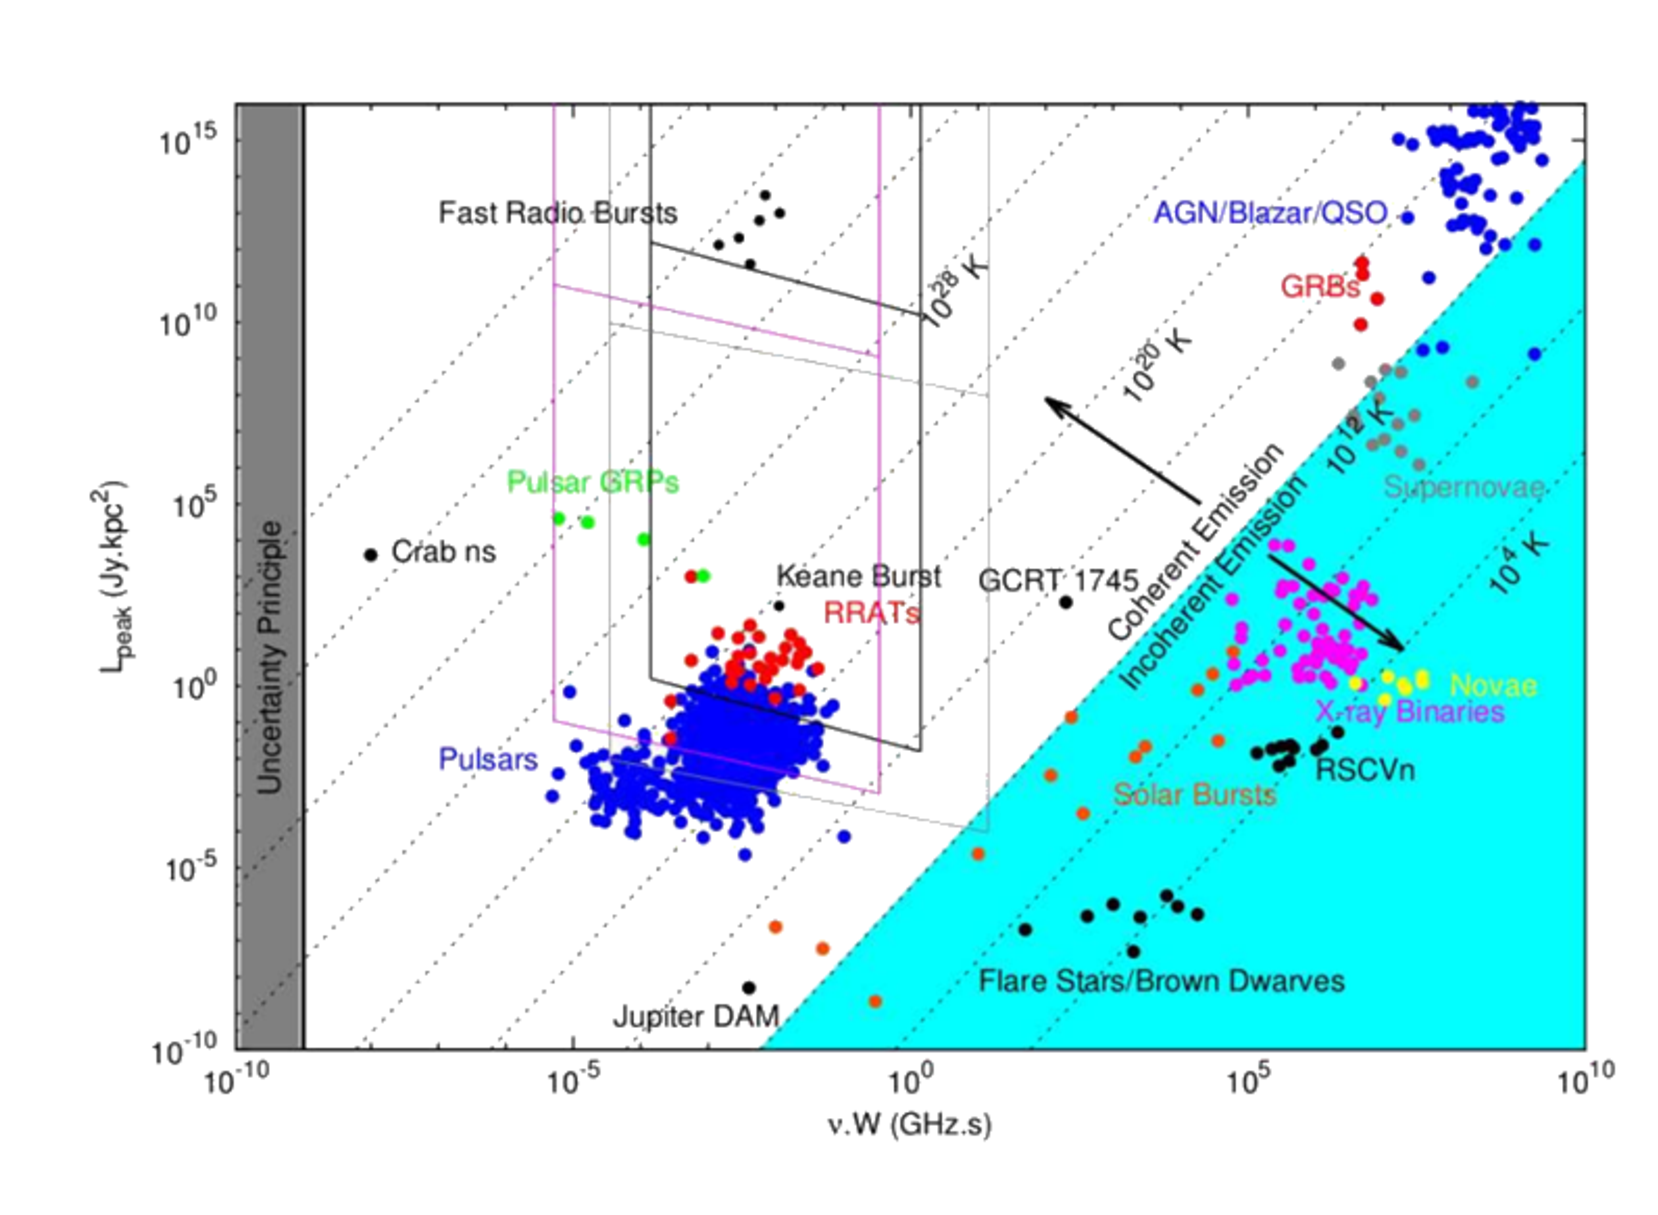
\includegraphics[width=0.9\textwidth]{transients/transients.phasespace.eps}
	\caption{突発・変動現象の相空間 (Cordes et al., in prep)。縦軸は光度変動の極大値、横軸はその変動のタイムスケールを意味し、各プロットは現象を表す。}
	\label{fig:transients.phasespace}
\end{figure}%
%コヒーレントな放射をする突発現象としては、例えばパルサーからのパルスやFRBが挙げられ、光度変動のタイムスケールは数秒以下と短い。
%変動している時間が短いため、それらは時系列の生データを解析することによって発見される。
%一方インコヒーレントな放射をする突発現象としては、例えばX線連星 (中性子星と恒星の連星など) からのバーストや超新星爆発が挙げられ、それらの多くは光度変動のタイムスケールが比較的長い。
%それらの変動は短くとも数日以上続き、たいていの場合数か月以上続くため、イメージング観測による画像データの中から発見されることが多い。

%%
\subsubsection{突発天体・変動天体の相空間}
%%
種々の突発天体をプロットした\Figref{fig:transients.phasespace}は、天体の光度$SD^2$とその変動の継続時間$W$が
\begin{align}
	SD^2 = 2 \pi k_\text{B} T (\nu W)^2, \quad \text{i.e.,} \quad
	\left( \frac{S}{\text{Jy}} \right) \left( \frac{D}{\text{kpc}} \right)^2 = 9.11 \times 10^{-18} \times
		\left( \frac{T}{\text{K}} \right) \left( \frac{\nu}{\text{GHz}} \cdot \frac{W}{\text{s}} \right)^2,
	\label{eq:transients.phasespace}
\end{align}
で関係付けられることに基づいている。
ここで$S$はフラックス密度、$D$は天体までの距離、$k_\text{B}$はボルツマン定数、$T$は輝度温度、$\nu$は観測周波数、$W$は変動の継続時間を表す。
%\footnote{電波の輝度温度とは、その電波が黒体から放射されたと見なしたときの、その黒体のもつ熱力学温度に等しい温度のこと。}
\Figref{fig:transients.phasespace}では縦軸に$SD^2~(=L_\text{peak})$、横軸に$\nu W$を取っており、複数の右上がりの直線は異なる温度$T$における\Eqref{eq:transients.phasespace}を図示したものである。

ここで\Eqref{eq:transients.phasespace}は以下のように導かれる。
レイリー・ジーンズ近似のもとで、電波天体の放射強度は $I_\nu \simeq 2\nu^2 k_\text{B} T / c^2$ と与えられる。
ここで$c$ は光速を表し、その他の量は前述のとおりである。
観測者から見た放射源の角度半径を $\theta_\text{src}$とすると、観測者の受信するフラックス密度$S$はその定義から
\begin{equation}
	S = \int_0^{2\pi} \td \phi \int_0^{\theta_\text{src}} \td \theta \sin \theta \cdot I_\nu \cos \theta
\end{equation}
で与えられる。
ここで実際の放射源の半径を $R_\text{src}$、観測者から放射源までの距離を$D$とすると、 $|\theta_\text{src}| \ll 1$であるから$\theta_\text{src} \simeq \tan \theta_\text{src} = R_\text{src} / D$と近似してよい。
また放射源の大きさ$R_\text{src}$ は変動の継続時間 $W$を用いて $R_\text{src} \simeq c W$として見積もることができるので、結局$\theta_\text{src} \simeq cW/D$と表せる。
したがってフラックス密度は
\begin{equation}
	S \simeq \pi \left( \frac{cW}{D} \right)^2 \cdot \frac{2\nu^2 k_\text{B} T}{c^2}
\end{equation}
と書け、これを変形すると\Eqref{eq:transients.phasespace}を得る。
以上のようにして、変動の継続時間 $W$ はその光度 $SD^2$ と関連付けられることがわかる。
この関係は、レイリー・ジーンズ近似、 $\theta_\text{src} \simeq \tan \theta_\text{src}$および$R_\text{src} \simeq c W$という3つの妥当な近似に基づいている。

以上のように\Figref{fig:transients.phasespace}は\Eqref{eq:transients.phasespace}に基づいた相空間を表しているが、その相空間は放射の輝度温度によって2つの領域 (白色と水色の領域) に分けられる。
地球で観測できる電波放射現象の多くは、インコヒーレントなシンクロトロン放射からなる。
しかしシンクロトロン電波の光子に電子が衝突する逆コンプトン効果によって、その光子はX線のエネルギーにまで叩き上げられ、結果的に電波の強度は制限されるという現象が起こる。
その制限された電波強度は、輝度温度にして$10^{12}~\text{K}$であり、もしある天体の輝度温度がその値を超えていた場合、その放射はコヒーレント放射かドップラー増幅されていることになる。
この輝度温度$10^{12}~\text{K}$の直線が、\Figref{fig:transients.phasespace}でコヒーレント放射の領域 (白色) とインコヒーレント放射の領域 (水色) を区切っている。

\Figref{fig:transients.phasespace}はすべての突発現象を網羅しているわけではないが、この相空間に広がる空白領域は、まだ発見されていない現象が数多く眠っていることを表している。
未知の現象があるということは、それを発見できれば新たな物理を開拓できる可能性があるということであり、科学はそのような未知の発見によって発展してきた。
したがって、\Figref{fig:transients.phasespace}の空白領域を埋めるような観測を積極的に行い、未知の現象を発見していくことが天文学者にとって重要な仕事となる。
その仕事を効率的に進めるには、高い感度と広い視野によって広範囲を探査することが必要であり、SKAはまさにそのような探査を可能とする。


\subsection{超新星} \label{transients.s1.sn}
超新星 (supernova; SN) は、星がその生涯の最期に爆発する現象であり、その爆発の実体として2つのシナリオが考えられている。
一方は、何らかの理由で白色矮星\footnote{恒星の場合、気体の圧力や核融合による輻射圧が重力とつりあって形状を保っており、白色矮星の場合は電子の縮退圧、中性子星の場合は中性子の縮退圧が、重力とつりあっている。}の質量が増大しチャンドラセカール質量\footnote{重力が電子の縮退圧を超える限界質量をチャンドラセカール質量とよび、それを超えた白色矮星は超新星爆発を起こす。}に達した時に、核暴走により白色矮星自体が爆発するというものである。
白色矮星質量を増大させる機構として、白色矮星と恒星の連星系において恒星のガスが白色矮星に降着するシナリオ、二つの白色矮星が重力波
放出を通し合体するシナリオが提案されている。
同様に白色矮星を起源とした核暴走として新星爆発が知られているが、この二つではその爆発の規模が大きく異なる。
新星爆発の場合は、白色矮星の表面上で一時的に核融合が暴走し爆発するだけで、白色矮星自体は爆発後も健在だが、超新星爆発の場合は白色矮星全体が爆発してしまい、後には何も残らず四散してしまうと考えられている。
もう一方のシナリオは、大質量星が自重を支えきれずに単独で重力崩壊し爆発するというものである。
大質量の恒星は内部に鉄などのコアをもつが、そのコアが重力崩壊を起こすと中心部に硬い原始中性子星がつくられ、それに衝突した物質がはね返って衝撃波をつくり爆発すると考えられている。% \citep[e.g.,][]{1994Natur.371..227N}。
このシナリオの超新星は、コアが重力崩壊することにちなんで、コア崩壊型超新星 (core-collapse supernova; CCSN) または重力崩壊型超新星とよばれる。
これらのシナリオは妥当なものだが、爆発に至る詳しいメカニズムはわかっておらず、コンピュータシミュレーションや観測事実の蓄積によって、その解明が試みられている。
超新星の分類は、歴史的にはスペクトルや光度曲線の特性によって行われ、\Figref{fig:transients.s1.sn}のように分類され命名されてきている。
連星系にある白色矮星の超新星爆発はIa型超新星に分類され、その他のIb型、Ic型、II型超新星はすべてコア崩壊型超新星である。
%例えばスペクトルに水素の吸収線が見られるものはII型に分類されるが、吸収線があるということは水素が豊富であることを示しており、\Figref{fig:transients.s1.sn}の右図のように水素が多く含まれた星が爆発したものと考えられる。
\begin{figure}[]
	\begin{minipage}{0.6\textwidth}
		\centering
		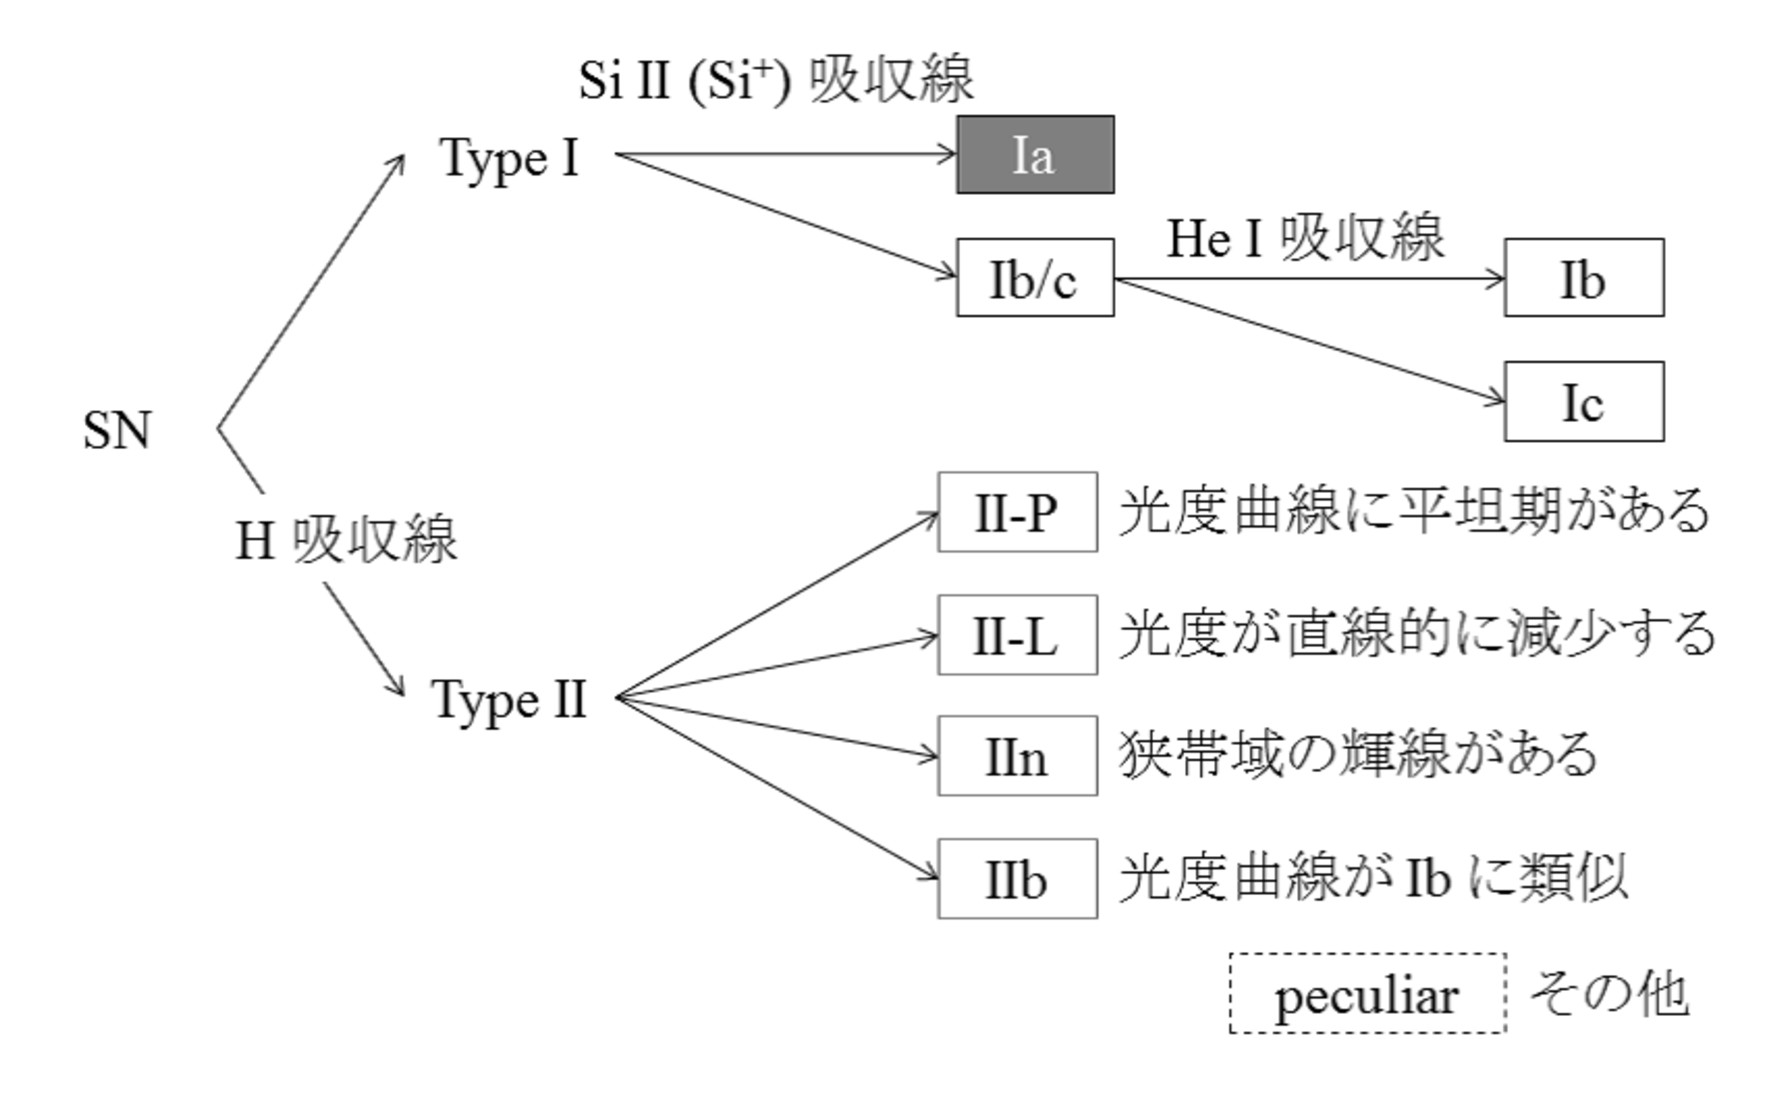
\includegraphics[width=\linewidth,clip]{transients/transients.s1.sn-class.eps}
	\end{minipage}
	\begin{minipage}{0.4\textwidth}
		\centering
		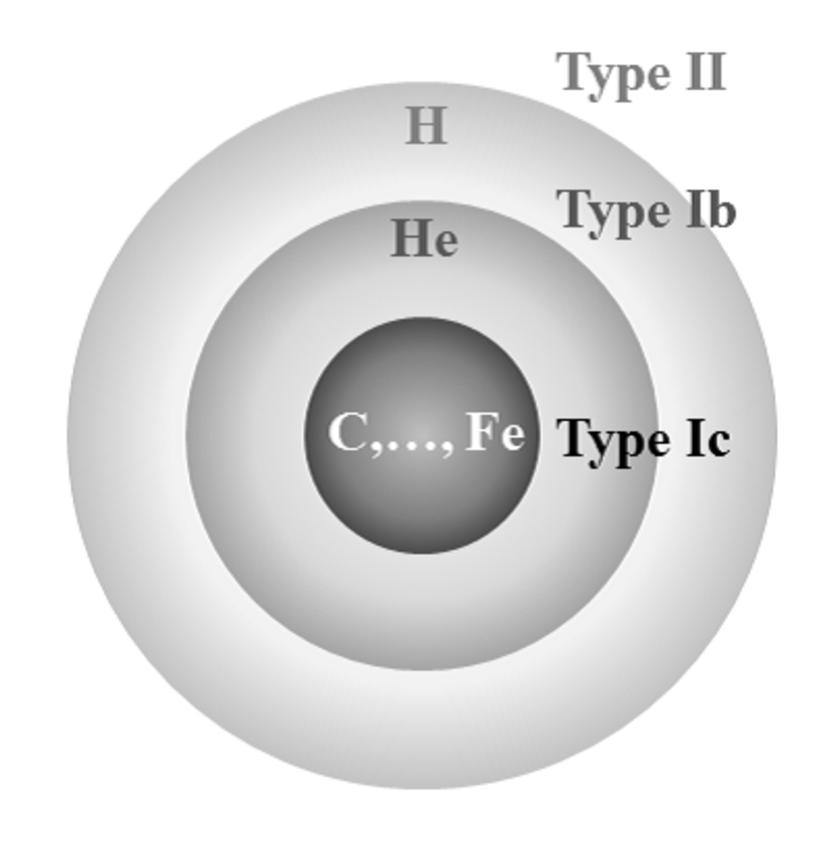
\includegraphics[width=0.7\linewidth,clip]{transients/transients.s1.ccsn.eps}
	\end{minipage}
	\caption{左図: 超新星の分類; 右図: コア崩壊型超新星となる以前の星の「たまねぎ構造」。}
	\label{fig:transients.s1.sn}
\end{figure}%

超新星爆発は主に光学望遠鏡によって発見され、電波望遠鏡で先んじて発見されたことはほとんどなかった。
%これは可視光域で明るいという理由の他に、光学望遠鏡は広い範囲を高い空間分解能で観測することに長けており、突発天体を発見しやすい装置であることも一因として挙げられる。
%またその探査では日本のアマチュア天文家による貢献も大きい。
%一方で従来の電波望遠鏡は、狭い範囲を極めて高い空間分解能で観測することに長けており\footnote{電波望遠鏡は、広い範囲を低い空間分解能で観測することにも長けている。}、それゆえ光学望遠鏡で発見された超新星を詳細に追観測することが主な役割だった。
SKAではこの状況を打破し、光学望遠鏡で発見された超新星の追観測のみならず、広い視野による広域探査によって電波帯域における超新星の発見を目指す。
また従来、Ia型超新星は暗すぎるために電波で検出されたことがないが \citep{2012ApJ...750..164C}、SKAによって初めてIa型超新星の電波観測が成功すると期待される。

超新星からの電波は、爆発の瞬間に放射されるのではなく、爆発前に星から噴出した物質に対して、爆発後に噴出した物質が衝突することによって放射されると考えられている。
したがって超新星を電波観測すると、爆発前後の星の状態を調べることができる。
また減光した後も、その噴出物は周りの星間物質と相互作用し続け、超新星残骸 (supernova remnant; SNR) とよばれる構造をなす。
その中では宇宙線の起源となる粒子加速が起こっていると考えられ、超新星残骸の電波観測によって他波長にわたる物理過程の解明が進むだろう。
可視光域で発見されている超新星のうち、従来の電波望遠鏡で観測できているものは一握りであるため、SKAによる高感度観測によって電波による観測サンプル数が増えれば、超新星の研究にとって大きなブレイクスルーとなるに違いない。

%%
%% GRB
%%
\subsection{ガンマ線バースト} \label{transients.s1.grb}
ガンマ線バースト (gamma-ray burst; GRB) は極めて遠方の銀河における突発的なガンマ線放射現象であり、その放射の継続時間によって2種類に分類され、継続時間が数秒以上と長いものを long-duration GRB、それ以下のものを short-duration GRB とよぶ。
GRBの大半は long GRB が占めており、他波長域でとても明るい残光が観測され、その実体は大質量星が重力崩壊したときの超新星爆発だと考えられている \citep{2006ARA&A..44..507W}。
またそのほとんどが星形成の盛んな銀河で発見される。
一方で short GRB は、中性子星やブラックホールなどの連星合体による爆発だと考えられ、星形成が活発ではない銀河で発見されている \citep{2007PhR...442..166N}。
連星合体は重力波源としてもっとも有力な候補でもあり、また\Secref{transients.s1.frb}で述べるFRBとの関連性も指摘されている \citep{2013PASJ...65L..12T}。

%%
%% Afterglow
%%
\subsubsection{GRB Afterglows}
GRBに伴う残光 (afterglow) は、ガンマ線が放射されてしばらく経ってから他波長域で明るく輝きだす現象である。
これは天体からジェットとして放出された物質が、星間物質に衝突することによって電磁波が放射されるというファイアーボールモデルでおおよそ説明でき \citep{1999PhR...314..575P}、GRB発生から残光として輝きだすまでの時間は場合によって異なる。
このGRB残光の光度曲線やスペクトル特性などから、GRBの発生機構や母銀河の構成成分などを知ることができ、そのためにはGRBの発生直後から他波長で継続して追観測することが重要となる。

それを実現するための追観測体制は世界的に整えられてきており\footnote{GRBの発見速報システムとしてNASAによるGRB Coordinates Network (GCN) があり、GRB発見後2秒以内にその位置情報などを他観測局へ速報し、迅速な追観測が可能になっている。}、ガンマ線観測衛星の発見速報を受けた他の観測局が、他波長でそれを詳細に追観測することが可能となっている。
それによってGRBの研究は最近10年程度で大きく前進し、超新星との関連性などいろいろな情報が得られ、先に述べたような実体の解明が進んでいる。
高感度なSKAでは、従来の望遠鏡では観測できなかった暗い電波残光をも観測できるため、この研究をさらに前進させGRBの統一描像の構築や、宇宙初期の様相の解明に大きく貢献するだろう。

%%
%% Orphan Afterglow
%%
\subsubsection{Orphan GRB Afterglows}
\begin{wraptable}{r}{2.5cm}
	\vspace{-4zh}
	\hspace{-4zw}
	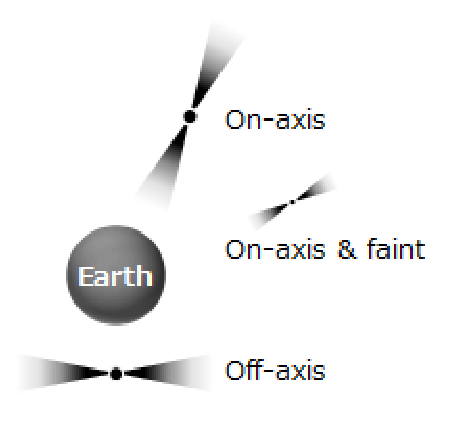
\includegraphics[width=3.5cm,clip]{transients/transients.GRB-afterglow.eps}
\end{wraptable}
GRBのガンマ線放射は高い指向性があり、その軸方向のみにガンマ線を放射するため、放射軸上に地球がなければガンマ線は観測されない。
一方でそれに付随する残光は指向性が高くないため、地球では残光のみが観測される、という状況を考えることができる \citep{1997ApJ...487L...1R}。
このような残光は親なし残光 (orphan afterglow) と呼ばれ、対応天体の見つからない電波トランジェントとして観測されうる\footnote{ガンマ線放射の軸が地球に向いていることを on-axis、向いていないことを off-axis と呼び、orphan afterglow は off-axis GRB afterglow と言い換えることができる。}。
\citet{2001ApJ...562L..55F}の見積もりによれば、99\% 以上のGRBで放射軸が地球から外れておりorphan afterglow のみが観測されると考えられるものの、従来の観測では候補天体が数例報告されているだけで、確定には至っていない。
SKAの広視野・高感度サーベイによって orphan afterglow を発見することができれば、GRB の物理の解明は大きく前進すると期待できる。
%

%

\subsection{ブラックホールによる星の潮汐崩壊} \label{transients.s1.tde}
超巨大ブラックホール (supermassive black hole; SMBH) のまわりを回る星々は、そのブラックホールから強い潮汐力を受け、もしその潮汐力の大きさが星の重力を越えると、その星は形状を保つことができず崩壊してしまう。
これを潮汐崩壊現象 (tidal disruption event; TDE) とよび、その際、まれにジェットを伴う爆発を起こし急激に光度を増す。

そのようなジェットを伴う潮汐崩壊現象は、特異的なガンマ線バーストとしてSwift衛星によって初めて観測され Swift J1644+57 (GRB 110328A) と命名された。
発見当初は起源がわからなかったが、その後、X線、赤外線、電波の追観測によって残光が観測され \citep{2011Sci...333..199L}、潮汐崩壊現象と考えられるにいたった \citep{2011Sci...333..203B}。
SKAはこの潮汐崩壊現象を数多く発見できると考えられ、銀河中心ブラックホールの物理に迫ることができるだろう。


%%\subsection{Magnetars (Anomalous X-ray Pulsars, Soft Gamma Repeaters)} \label{transients.s1.magnetars}

\subsection{Fast Radio Bursts (FRBs)} \label{transients.s1.frb}
銀河系外からの電波パルスは、1930年代に電波天文学が拓かれて以降近年に至るまで、発見されてこなかった。
つまり\Tabref{tb:frail-classification}の左上の欄は、近年まで空白のままであった。
しかしついに2007年、銀河系外起源と思われる電波パルスがオーストラリアParkes 64~m 電波望遠鏡によって発見された \citep{2007Sci...318..777L}。
そのパルスは幅数ミリ秒と短寿命かつ大強度であり、さらに発見された位置が高銀緯にも関わらず分散測度 (dispersion measure; DM) が極めて大きいことから、その起源は銀河系外の高エネルギー天体だと考えられた\footnote{
最初に発見されたFRB~010724 (Lorimer burst) は、パルス幅が $W=5~\text{ms}$、フラックス密度が $S_{1.4~\text{GHz}}=30~\text{Jy}$、また発見された位置が銀緯$b = -41.8\arcdeg$、パルスの分散測度は$\text{DM} \sim 375~\text{pc}~\text{cm}^{-3}$であった。
それから推定される地球からの距離はおよそ500~Mpcと考えられ、また遠くとも1~Gpc以内の天体だと考えられている。
}。
さらにパルス放射はその1発限りであり、それ以降同じ場所からの電波放射は確認されていない。

このような現象は従来報告されておらずその信憑性が疑われたこともあり、しばらくは発見者の名前をとってLorimer burst と呼ばれていたが、同様のパルスが \citet{2011MNRAS.415.3065K} および \citet{2013Sci...341...53T} によって新たに5例発見され、この銀河系外からの電波パルスは fast radio bursts (FRBs) と呼ばれるに至った。
このFRBの起源はわかっておらず、そもそもPerytonと命名されている地球起源の謎のノイズ \citep{2011ApJ...727...18B} との区別も明確ではない。
しかしその後、オーストラリアから遠く離れたプエルトリコのArecibo 300~m 電波望遠鏡によって同様のFRBが1例発見され \citep{2014ApJ...790..101S}、FRBが宇宙起源の天体現象であることの信頼性は非常に高まっている。
起源天体のモデルとしては多くの説が唱えられており、
銀河系内からの放射では説明しにくいことが様々な研究で示されている \citep[e.g.,][]{2014ApJ...797...70K}。
%ただし一方で系内起源を主張する研究もあり \citep[e.g.,][]{2014MNRAS.439L..46L}。
%例えば中性子星連星の合体に伴う電波放射モデルが提案されており (\citealt{2013PASJ...65L..12T})、合体に伴う重力波放射との一致性が確認されれば宇宙物理学に大きな影響を与えるだろう。


%%
%% Unknowns
%%
\subsection{未知の突発天体} \label{transients.s1.unknowns}
本節では電波帯域でのみ観測され、他の波長帯域やあるいは電波帯域ですら対応天体が見つかっていないような未知の突発天体について紹介する。
併せて、既知の天体と同定はできているものの、その放射過程が未解明な天体についても述べる。
その紹介にあたっては観測方法に着目した\Tabref{tb:frail-classification}の分類法に従い、その天体が銀河系外か系内にあるか、短時間変動か長時間変動か、という4種類に分けて述べる。

%%
%% ss1
%%
\subsubsection{種類1: 銀河系内の短時間変動天体}
銀河系内の天体に起源を持ち、変動の継続時間が数秒以下のパルスを発する天体として代表的なものはパルサー、つまり自転する中性子星である。
それらパルサーの中でも、Crab nanoshots や RRATs といった特殊なパルス放射現象が報告されおり (次項参照)、それらの現象は突発天体研究においても興味深い研究対象である。
また銀河系内でパルス状の電波放射をする天体としては中性子星のみが知られており、それ以外の系内天体で電波パルスは観測されていないが、今後、中性子星起源とは考えられないような電波パルスが観測されることもあるかもしれない。
そのような未知の突発現象観測には、従来の望遠鏡を越える感度と高い時間分解能、そしてデータ解析コンピュータの計算速度が要求される。

%%
\paragraph{Crab Nanoshots}
電波パルサーの中には、通常のパルス放射とは異なる放射をするパルサーがあることが、近年明らかになってきている。
Crabパルサーから放たれるパルスは、そのパルス幅が 3~ms、パルス周期が 33~msであり、そのフラックス密度は平均して 14~mJyである。
一方で時折、大強度のジャイアントパルスを放つことがあり、そのフラックス密度は 1~MJy に達することもある。
このジャイアントパルスの中で、パルス幅が通常よりも極端に短くなる現象がArecibo 電波望遠鏡を用いた周波数 9.25~GHz の観測によって明らかとなった。
そのパルス幅は観測の時間分解能 0.4~ns より短く、フラックス密度は 2~MJy という極めて短寿命で大強度のパルスであり、nanoshots と呼ばれた \citep{2003Natur.422..141H,2007ApJ...670..693H}。
そのパルスの放射源の大きさは 12~cm、輝度温度は$10^{41}~\text{K}$と見積もられ、高エネルギーかつコンパクトな天体現象である。

発見者らはこのnanoshotsを説明できる唯一のモデルとして \citet{1998ApJ...506..341W} によって提示されたプラズマ乱流モデルを挙げているが、その放射機構は必ずしも解明されていない。
また同様にパルス幅が短くなる現象は他のパルサーでは確認されておらず、現状ではCrabパルサーに特有の現象である。
さらにはジャイアントパルスでのみ起こるのか、本質的には通常のパルスでも起こっているが感度不足で検出できていないだけなのかという点もわかっていない。
SKAを用いた高感度観測によってnanoshotsについてより詳しい知見が得られれば、パルサー磁気圏の研究が大きく進むと期待できる。

%%
\paragraph{RRATs}
通常のパルサーとは異なるパルス放射天体としては、Parkes 64~m 電波望遠鏡で発見された rotating radio transients (RRATs) が挙げられる \citep{2006Natur.439..817M}。
このRRATsはパルサーと同様に強い磁場を持つ中性子星が起源だと考えられているが、パルサーの周期的なパルス放射とは異なり、その放射は散発的で放射機構は明らかとなっていない。
SKAを用いてRRATsを高感度で観測すれば、その散発性についてより詳しい議論が可能になるだろう。


%%
%% ss2
%%
\subsubsection{種類2: 銀河系外の短時間変動天体}
銀河系外からの電波パルスは、\Secref{transients.s1.frb}で述べたFRBのみである\footnote{FRBは\Secref{transients.s1.frb}で述べたように銀河系内を起源とする説もあり、必ずしも系外天体として見解が一致しているわけではない。}。
FRBは従来予想もされていなかった現象であり、発見当初はそれほど大きな注目を集めていなかった。
しかしその後アーカイブデータの解析によって続々と発見されたため、現在は大きな注目を集め、SKAによる重要なサイエンスの一部を担うに至っている。
FRBのような未知の天体は、まだ宇宙に多く眠っていると考えられ、それらを発見するには柔軟な観測システムが必要となり、SKAはそれを実装しなければならない (\Secref{transients.s2.fender})。

%%
%% ss3
%%
\subsubsection{種類3: 銀河系内の長時間変動天体}
銀河系内を起源とした数秒以上の長時間変動を示す天体は数多くあり、例えば\Tabref{tb:frail-classification}に挙げた恒星フレアやメーザーバースト、X線連星における電波バーストなど多種多様である。
それらのほとんどは対応天体が見つかりやすく、起源がわかっているものが多い。

一方で対応天体が同定されていないものもあり、例えば\citet{2005Natur.434...50H} が銀河中心近傍に発見した周期的なバースト現象が挙げられる。
このバーストはフラックス密度が 1~Jy、1回のバーストの幅が 10 分でそのバーストが 77 分周期に5回現れるという特異的な突発現象であり、VLA を用いた観測によって発見された。
この天体は GCRT J1745-3009 と名付けられ\footnote{接頭辞 GCRT は Galactic Center Radio Transient の頭文字をとったものである。}、対応天体は見つかっておらず放射機構も不明である。
しかしその後の追観測によって同じ場所から同様のバーストが観測され、\citet{2010ApJ...712L...5R} によって偏波情報が明らかとなった。

その情報などから起源についていくつかのモデルが発案されており、その中には、一時的にパルス放射が消える nulling pulsar (\citealp{2005Natur.434...28K})、中性子星連星 (\citealp{2005ApJ...628L..49T})、白色矮星 (\citealp{2005ApJ...631L.143Z})、歳差運動するパルサー (\citealp{2006MNRAS.365L..16Z})、恒星フレア (\citealp{2010ApJ...712L...5R}) などがある。
以上のように起源について多くのモデルは考えられているが、それらについて確証は得られていない。
このような数分スケールのバースト現象の探査は大規模には行われておらず、SKAにおいてもデータ解析システムに対して同様のバーストを効率的に探査する機能を要求する必要がある。

%%
%% ss4
%%
\subsubsection{種類4: 銀河系外の長時間変動天体}
銀河系外における長時間変動を示す天体のうち、対応天体が見つかりにくく未知天体と認識されるものとして代表的なのは、orphan GRB afterglow (\Secref{transients.s1.grb}) や TDE (\Secref{transients.s1.tde}) であろう。
GRB残光や超新星爆発に代表される突発現象は、電波帯域では増光は急激だが減光は緩やかで、その継続時間は数か月以上に及ぶものも多い。
一方、変動の継続時間が数か月以下で、起源が未知の突発天体がいくつか報告されている。

例えばVLA のアーカイブデータからは4つの候補天体が発見されており、特にRT~19920826と命名されたものについては検出状態も良好であった \citep{2007ApJ...666..346B,2012ApJ...747...70F}。%
同様の突発天体は早稲田大学の那須パルサー観測所においても発見され、WJN~J1443+3439と命名された天体があるが、その起源については恒星フレアやAGNフレアが示唆されているものの、必ずしもわかっていない \citep{2007ApJ...657L..37N,2014ApJ...781...10A}。
そのような未知の突発天体を探査し、\Figref{fig:transients.phasespace}の空白領域を埋めるには、広い視野を高感度で探査し、さらに様々な時間分解能でデータ処理するための解析システムが必要になる。

%%\subsubsection{LOFAR Transients を加筆}


%%
%% Section 2
%%
\section{国際SKAのサイエンス}\label{transients.s2}
国際SKAサイエンスブックでは「The Transient Universe」という領域区分があり、突発天体に関する論文はその領域に集録されている。また周辺領域の研究としてパルサーに関する論文もあり、それらは「Fundamental Physics with Pulsars」という領域に集録されている。本節では「The Transient Universe」に集録されている12の論文について紹介していく。表\ref{c09.s2.t1}には12の該当論文をリストした。次小節からはそれぞれの概要を紹介していく。他の国際科学検討班のポリシーとは異なり、これらの論文は草稿段階から2015年1月まで非公開であった。そのため準備期間が無く、詳細な解説はできなかった。突発天体科学研究班では、今後これらの論文について、時間をかけてより深く検討を進める予定である。

\begin{table}[htbp]
\begin{center}
\caption{国際SKAサイエンスブックの突発天体領域論文一覧$^*$}
\small
\begin{tabular}{llp{28zw}}
\hline\hline
\noalign{\smallskip}
ID$^\dag$ & PI & Title\\
\noalign{\smallskip}
\hline
\noalign{\smallskip}
The Transient Universe &&\\
051 & R. Fender & The Transient Universe with the Square Kilometre Array \\
052 & D. Burlon & The SKA View of Gamma-Ray Bursts \\
053 & S. Corbel & Incoherent transient radio emission from stellar-mass compact objects \\
054 & I. Donnarumma & SKA as a powerful hunter of jetted Tidal Disruption Events \\
055 & J.P. Macquart & Fast Transients at Cosmological Distances with the SKA \\
056 & L. Amati & The SKA contribution to GRB cosmology \\
058 & H.E. Bignall & Time domain studies of Active Galactic Nuclei with the Square Kilometre Array \\
060 & M. Perez-Torres & Core-collapse and Type Ia supernovae with the SKA \\
062 & T. O'Brien & Thermal radio emission from novae \& symbiotics with the Square Kilometre Array \\
064 & L. Wang & Investigations of supernovae and supernova remnants in the era of SKA \\
065 & P. Wilkinson & The Unknown Unknowns \\
066 & W. Yu & Early Phase Detection and Coverage of Extragalactic and Galactic Black Hole X-ray Transients with SKA \\
\noalign{\smallskip}
\hline
\noalign{\smallskip}
\multicolumn{2}{l}{\small $^{*}$ArXiv未投稿含む} & \\
\multicolumn{2}{l}{\small $^\dag$ PoS (AASKA14) ID} & \\
\end{tabular}\label{c09.s2.t1}
\end{center}
\end{table}

\subsection{SKAによる突発天体探査}\label{transients.s2.fender}
第~\ref{transients.s1}節および次節以降で述べるように、宇宙における突発現象は極めて高エネルギーな現象が元になっていると考えられ、その観測的研究によって新たな物理が開拓される可能性を秘めている。
ただし、突発現象は宇宙のいつどこで起こるかということが予測することができないため、探査のみをやみくもに続けることはリスクが高い。
しかしこのことは裏を返せば、突発天体の探査は他の目的の観測と並行して実施できるということである。
また突発現象は、初期の増光段階と時間経過後の減光段階で、電波放射の物理過程が異なることもあり、現象が発生した直後から継続して追観測することが重要である。
そのような特徴や課題をもつ突発現象の観測的研究では、以下の二つの機能をSKAに実装することが重要な鍵となる:
\begin{itemize}
	\item[(1)] 他の目的による観測と共存・並行して運用できる、突発天体の探査観測システム、
	\item[(2)] 突発天体が発見された際に、それを即時的・自動的に追観測するシステム。
\end{itemize}
本節ではこの二つの機能について紹介する。

%%
\subsubsection{SKAへの要求 (1): 他の観測と共存する突発天体探査システム}
%%
探査によって突発現象を発見できるかどうかは確率によって評価できるが、多かれ少なかれ運に左右される。
しかし一方で、探査は他の目的の観測と並行して実施することができ、多大な観測時間を費やすことができるという大きなメリットがある。
観測時間が多ければ多いほど突発現象を発見できる確率は上がるため、その探査システムを他の観測と共存できるように構築することで、効率的に探査ができるようになり大きな科学成果を期待できる。

そのようなシステムとして、例えば図~\ref{fig:transients.fender.commensal}に示すようなシステムをアフリカのMeerKATに実装することが提案されている (Armstrong et al., in prep)。
この共存システムは、観測データの処理経路を分岐させ、一方を本来の観測のために使用し、もう一方を突発天体のリアルタイム探査に使用するというものである。
図~\ref{fig:transients.fender.commensal}は観測データの流れと処理過程を示しており、図左上の相関器 (correlator) から処理が始まる。
通常の観測では、相関器から出力される電波干渉計のデータに対して図右方向に向かってさまざまな解析処理を施し、最終的に輝度分布画像を得る。
その観測には通常数時間以上を費やし、その長時間の観測データを後日取りまとめる場合が多い。
一方で突発天体は、その変動のタイムスケールが観測時間よりも短い可能性があり、またその追観測には即時性を要する。
そのため突発天体探査は通常観測だけでは不十分であり、リアルタイムにデータ処理を行う必要がある。
そこで通常観測と共存する形で処理経路を分岐させ、即座に簡易的な画像データを得て天体の光度変動を検出する。
それを行うのが図~\ref{fig:transients.fender.commensal}の左半分に示されるシステムである。
もし突発天体が検出されれば、自動的にその情報を VOEventNet と呼ばれる突発天体の発見速報ネットワークに通報する。
その通報によって、世界中の他の観測局がその突発天体を追観測することができれば、その起源や放射機構について詳しい情報が得られることだろう。
\begin{figure}
	\centering
	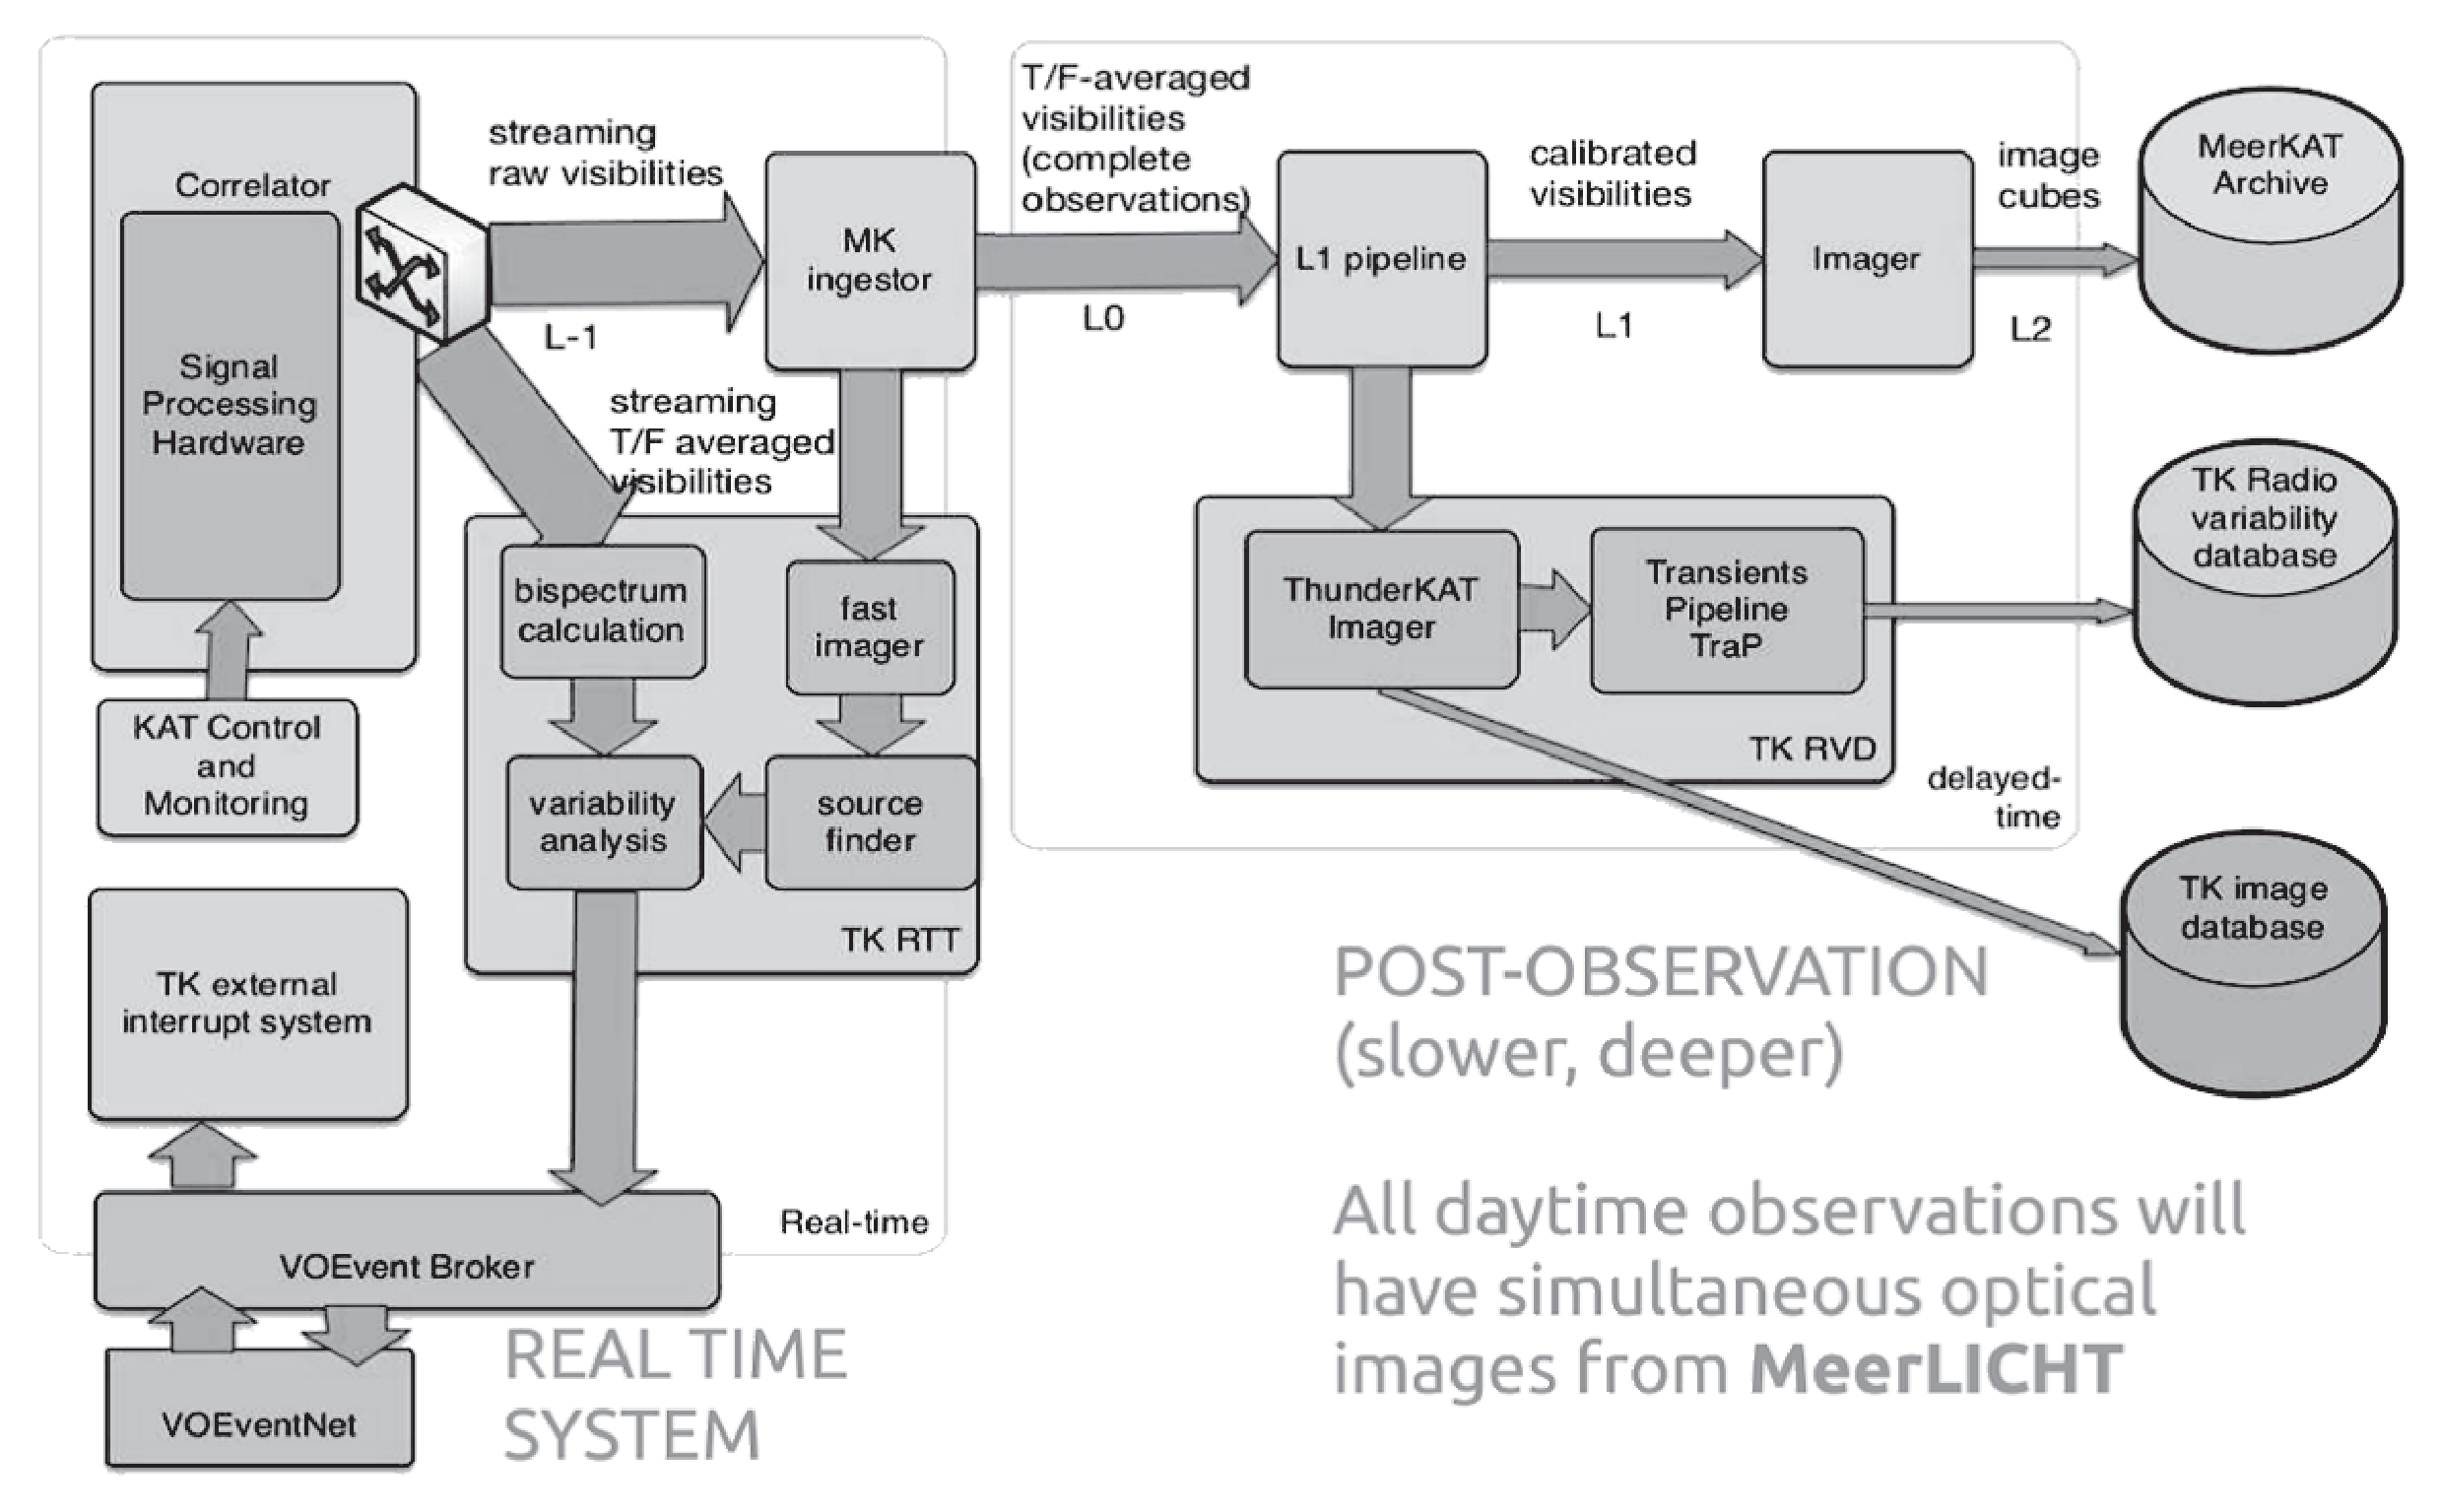
\includegraphics[width=12cm]{transients/transients.s2.fender.commensal.eps}
	\caption{他の観測と共存した突発天体探査システム。}
	\label{fig:transients.fender.commensal}
\end{figure}%

%%
\subsubsection{SKAへの要求 (2): 突発天体発見時の自動的な追観測システム}
%%
突発天体の観測的研究に重要なもう一方のシステムは、他の観測局によって発見された突発天体、あるいはSKA自身によって発見した突発天体を、自動的に追観測するというものである。
このようなシステムは既にイギリスのArcminute Microkelvin Imager Large Array (AMI LA) に実装されており、ガンマ線観測衛星Swiftで発見されたガンマ線バーストを約8時間後に追観測することに成功している \citep{2013MNRAS.428.3114S,2014MNRAS.440.2059A}。
この結果得られた電波帯域での光度曲線から、ガンマ線バーストのリバースショック (星間物質から噴出物の方向に伝わる衝撃波) による電波放射が、世界で初めて確認された。
同様にSwiftの速報によって、地球近傍の連星系 DG~CVn からのガンマ線フレアを6分以内に追観測した結果、電波帯域でも大きいフレアが確認され、広い周波数帯域でのコインシデンスが得られている。
しかし数日後には元の明るさに戻ってしまい、そのようなタイムスケールの短い突発現象を詳細に観測するためには、世界規模で即時的な追観測を行うことが重要である \citep{2015MNRAS.446L..66F}。
SKAにおいても同様のシステムを実装すれば、突発天体の研究にブレイクスルーを起こすことができるだろう。

%%
\subsubsection{まとめ}
%%
突発天体の観測的研究には、SKAに前述の二つのシステムを実装することが重要である。
SKAは広い視野と高い感度を兼ね備えており、さらにそのシステムが実装されれば、電波帯域での変動天体や突発天体を数多く発見することができるだろう。
その発見は、究極の宇宙物理を議論できる場所に、人類を導いてくれるはずである。
突発現象というのは宇宙の、とりわけ深宇宙の灯台であり、その観測によって新しい物理を開拓できるに違いない。


%\setcounter{section}{1}\section{国際SKAサイエンスブックの紹介} \label{c09.s2}

%%%%%%%%%%%%%%%%%%%%%%%%%%%%%%%%%%%%%%%%%%%%%%%
%%%%%%%%%%%%%%%%%%%%%%%%%%%%%%%%%%%%%%%%%%%%%%%
\subsection{ガンマ線バースト}
\label{c09.s2.ss2}

\paragraph{GRB電波残光の観測の現状}

GRBは宇宙で起こる極限現象のひとつであり、基礎的な物理過程を探る自然界の実験場の役を果たすだけではなく、おそらく極限の赤方偏移に至るまでの宇宙の星形成率をトレースし宇宙史に渡る銀河間物質の構成を示すだろう。
GRBの電波観測はGRBの物理特性を決定する中心的な部分を担う。
しかしながら現在までのところ、GRBの電波観測は大抵ガンマ線検出天体のフォローアップ観測に限られてしまっている。

\paragraph{GRB電波残光のSKA観測の見込み}

SKAは、Phase~1 の初期科学段階で高周波帯域で数百の天体をフォローアップし、GRB残光の研究を大幅に進展させるだろう。
\skamid{1}のBand~4 (4~GHz) と Band~5 (9.2~GHz) はとりわけGRB残光のような突発天体現象の探知に向いているだろう。
時間進化する放射スペクトルの光学的厚みの遷移をサンプルしながら、電波残光のピークを探知する。
そして放出物が非相対論的な速さに減速する時間までの残光を追跡できる。
SKA2では全GRBの25\% についてその減速までの残光を観測することができるだろう。
これはGRBの真のエネルギー割当量、周辺の密度分布、そして衝撃波の物理について重要な知見を与えるに違いない。
SKAは、ジェットが地球を向いていないGRBからの orphan afterglow を日常的に探知できるようになるだろう。
\skasur{1} の深い全天サーベイは、毎週300イベント程度のorphan afterglowを検出するだろう。その検出率はSKA2では1000を超えると予想される。

%%%%%%%%%%%%%%%%%%%%%%%%%%%%%%%%%%%%%%%%%%%%%%%
%%%%%%%%%%%%%%%%%%%%%%%%%%%%%%%%%%%%%%%%%%%%%%%
\subsection{太陽質量コンパクト天体からのインコヒーレントな突発的電波放射}
\label{c09.s2.ss3}

\paragraph{太陽質量コンパクト天体と電波放射}

物質降着するコンパクト天体によるジェット形成とアウトフローは、物質降着と物質放出の間の関係によって決まる。
この放出過程におけるインコヒーレントなシンクロトロン放射は、ブラックホール、中性子星、そして白色矮星を含む多くの降着連星天体で観測されている。

\paragraph{電波観測から分かること}

散発的なアウトバースト中の電波放射の進化をモニタリングすることは、ジェットの立ち上がりについて重要な知見を与え、また、より高周波帯での観測と合わせれば、ジェットと降着円盤の潜在的な関係を解き明かすことになるだろう。
電波観測によって、マグネターの巨大フレアなどの爆発的イベントも含めたジェットやアウトフローの、運動学的なフィードバックを定量化することができれば、星周物質への重要性も示すことができる。

\paragraph{感度への期待}

SKAの高感度は、明るいエディントン限界のアウトバースト状態から、元々暗くて詳細な研究ができなかった低光度の鎮静したレベルまで、質量降着する太陽質量コンパクト天体のモニタリングを可能にし、新しいパラメータ空間を切り拓くだろう。
鎮静した質量降着ブラックホールの国勢調査は、連星系の進化過程にも制限を与えるだろう。
これまでのブラックホールジェットの調査を中性子星や白色矮星のより暗いジェットへと拡張することを可能にすることで、SKAはジェット形成におけるコンパクト天体の役割を決めるための比較研究を可能にする。
SKAの高感度と広視野そしてマルチビーム能力を駆使すれば、観測しうる近傍宇宙($\sim$15 Mpc以内)の全ての「明るいフレア天体」の探知とモニタリングが可能となる。
それは初代クェーサーの成長への重要な示唆と共に、質量降着率が極めて高いコンパクト天体におけるジェットの特性について、我々に新たな知見を与えるに違いない。
そこには超高輝度X線源 (ultraluminous X-ray source; ULX) の電波対応も含まれる。

\paragraph{SKA観測の見通し}

シンクロトロン過程は、高周波にて早くピークを迎え、またフラックス密度が大きいので、以上のような研究は\skamid{1}の高周波帯Band~4 と 5 で、最も効率よく観測できるだろう。
\skamid{1} の高い感度があれば、太陽質量ブラックホールや球状星団内の中間質量ブラックホールの存在が想定される領域から、Bondi-Hoyle降着の進む孤立した鎮静ブラックホールを検出することもできるだろう。

%%%%%%%%%%%%%%%%%%%%%%%%%%%%%%%%%%%%%%%%%%%%%%%
%%%%%%%%%%%%%%%%%%%%%%%%%%%%%%%%%%%%%%%%%%%%%%%
\subsection{ジェットを伴う潮汐崩壊現象の強い狩人としてのSKA}
\label{c09.s2.ss4}

\paragraph{潮汐崩壊現象}

超巨大ブラックホール (SMBH) による星の潮汐崩壊現象 (TDE) の観測的な帰結は、鎮静したSMBHを発見することを可能にし、それらの質量関数を制限することにつながる。
それ以上に、かつては活動的ではなかった銀河におけるジェットを伴った潮汐崩壊を観測することは、初期段階、言い換えれば「汚れのない」環境での、ジェット形成と進化を研究するという新しい意味をもたらす。

\paragraph{潮汐崩壊現象の観測}

数から数十の潮汐崩壊は1999年以降発見されてきているが、ジェットを伴った潮汐崩壊はたった2つだけ硬X線によって発見された。そしてそのうちのただ1つ、Swift J1644+57だけが潮汐崩壊現象という解釈をさらに支持するような精密位置決定がなされた。これら2イベントだけでは上記の科学的問題に取り組むには不十分であり、サンプルをもっと圧倒的に増やさなければ取り組めない。

\paragraph{SKAへの見通し}

X線は実際に観測された電磁波帯にも関わらず、現在または近い将来のX線装置はジェットを伴った潮汐崩壊現象を発見する最有力装置とはならないだろう。
それらはせいぜい年間で数から数10のイベントを与えるのみと考えられる。
実際の所、潮汐崩壊現象を検出し多波長フォローアップのトリガーをかけるためのベストな戦略は、SKAを用いることである。
SKAは年間で数100のイベント、赤方偏移で$z\simeq 2$程度までのイベントを発見できるだろう。
とはいえ、電波とX線のシナジーは原理的に、ジェットを伴った潮汐崩壊現象の絶対的な発生率、それらのジェットのパワー、群ローレンツ因子、ブラックホール質量関数、といった重要な物理量を制限することができる。
そしておそらく、質量が$10^5~\text{M}_\odot$以下の中間質量ブラックホールを見つけることができるだろう。
最終的に、Large Synoptic Survey Telescope (LSST) などの可視光サーベイとSKAを比べることで、ジェット発生効率をより直接的に制限することができる。

%%%%%%%%%%%%%%%%%%%%%%%%%%%%%%%%%%%%%%%%%%%%%%%
%%%%%%%%%%%%%%%%%%%%%%%%%%%%%%%%%%%%%%%%%%%%%%%
\subsection{宇宙論的距離の早い突発現象}
\label{c09.s2.ss5}

\paragraph{早い突発現象の活用}

宇宙論的距離にわたって探知しうる電波バーストは、銀河間物質 (IGM) と銀河間磁場、そして時空そのものの強い証拠の一つとなる。
それらの分散測度 (DM) は、いわゆる近傍赤方偏移宇宙の「ミッシングバリオン」を解く鍵となり、銀河形成・フィードバックモデルのキーパラメータである銀河ハロープロファイルの初測定を可能にするだろう。
電波バーストは赤方偏移$z\simeq 2$を超えるところでの宇宙のものさしとして使うことができ、ダークエネルギーの状態方程式のパラメータ$w(z)$を、Ia型超新星で測られている赤方偏移をはるかに超えて制限することができる。
これらの科学成果は、可視光フォローアップでホスト銀河の赤方偏移を得るのに十分な1\arcsec 以内に位置精度が収まる、およそ$10^4$のFRBサンプルによって実現できる。
重力波イベントはSKA1-LOW帯域でコヒーレントな放射をすると仮定すると、宇宙論的な距離のFRBの位置決定は宇宙論的な標準サイレンとして使うことができる。

\paragraph{SKAへの見込み}

以上のような研究を実施するためには、発見したFRBのDM, RM, SMと比べられるように、FRBのホスト銀河を特定し、その赤方偏移を測定しなければならない。
そしてこれは、半径3~km 内に全アンテナの80\% を集めたコンパクト構成による集光デザインで実現でき、また高時間分解の信号処理機器を伝送路上に設置することが求められる。

%%%%%%%%%%%%%%%%%%%%%%%%%%%%%%%%%%%%%%%%%%%%%%%
%%%%%%%%%%%%%%%%%%%%%%%%%%%%%%%%%%%%%%%%%%%%%%%
\subsection{ガンマ線バーストを用いた宇宙論へのSKAの貢献}
\label{c09.s2.ss6}

\paragraph{GRB宇宙論}

ガンマ線バースト (GRB) の光度は一定ではなく標準光源ではないが、宇宙の幾何学と膨張率を測るツールとして注目されている。
それはFRBの$10^{53}~\text{erg/s}$を超える膨大な光度と、$z=8$を超える高赤方偏移というユニークな組み合わせによる。
近年、GRBを標準化し宇宙論パラメータ推定に使うために、いわゆる$\nu F_\nu$スペクトルのピーク光子エネルギーと、放射の強度 (放射されたエネルギーないし光度) の関係を活用するいくつかの試みがなされた。
これらの研究によって、既存のGRBデータから$\Lambda$CDM宇宙模型の物質パラメータ$\Omega_\text{M}\sim 0.3$が導き出された。
現在そして次世代のGRB観測 (Swift, Fermi, SVOM, UFFO)\footnote{SVOM: Space Variable Objects Monitor; UFFO: Ultra-Fast Flash Observatory.} により期待される結果から、ダークエネルギーの特性と進化の手がかりをつかむことが可能となるだろう。

\paragraph{SKAへの見込み}

SKAを用いたGRBの電波観測および他波長観測の結果から、従来は得られなかったGRBの特徴が明らかとなるだろう。
GRBの研究はSKAのその他の天体に関する主要科学計画の観測を補い、SKAの主要科学目的のいつくかに重要な貢献をすると期待できる。

%%%%%%%%%%%%%%%%%%%%%%%%%%%%%%%%%%%%%%%%%%%%%%%
%%%%%%%%%%%%%%%%%%%%%%%%%%%%%%%%%%%%%%%%%%%%%%%
\subsection{活動銀河核の時間領域研究}
\label{c09.s2.ss7}

\paragraph{AGNの時間領域研究の背景}

活動銀河核 (active galactic nucleus; AGN) の電波変動の観測は、内在的な変動と外来的な変動の両方を明らかにすることができる。
内在的なものは衝撃波・フレア・超巨大ブラックホール周りの放射の変化、外来的なものはたとえば天の川銀河の構造による散乱が原因である。
そのような星間散乱はマイクロ秒角の空間分解能で放射領域の構造を示す。
現在までのAGN観測は、長期間モニターされ続けた天体が少ない、あるいは、モニター数は多いが時間分解能に乏しい、といういずれかの問題を抱えていた。

\paragraph{SKAへの見込み}

SKAを用いることによるサーベイ能力の劇的な向上は、毎日かそれ以下の頻度で10万個のAGNの精密な外観モニター研究を可能にする。
変動の統計、特に多周波同時観測は、AGNのクラス、光度、そしてジェット指向性という多くの問題を解決し、質量降着の物理を示すだろう。
また星間物質による電波散乱の原因となる構造を、詳細に解明できるだろう。

%%%%%%%%%%%%%%%%%%%%%%%%%%%%%%%%%%%%%%%%%%%%%%%
%%%%%%%%%%%%%%%%%%%%%%%%%%%%%%%%%%%%%%%%%%%%%%%
\subsection{コア崩壊型超新星とIa型超新星}
\label{c09.s2.ss8}

\paragraph{コア崩壊超新星}

コア崩壊型超新星 (core-collapse supernova; CCSN) からの電波放射の系統的な調査はいまだなく、狙いをつけた調査、つまり近傍宇宙のいくつかの可視光で発見されたCCSNからの電波のみが観測されてきた。
可視光での調査はダスト減光により大部分のCCSNを見損なう。
ゆえにCCSNの電波での調査は覆い隠されていない完全な近傍宇宙の星形成率を与えることに有望である。
SKAはこの領域の調査に、他の目的の観測に「相乗り」する形で、広視野のブラインドサーベイを行うことが重要である。
計画中の VLA Sky Survey (VLASS) が最大でも数10個のCCSNを発見する見込みに対して、\skasur{1}はたった1年で数100個のCCSNを発見し、SKA1の10倍の感度を持つSKA2では近傍宇宙で数千個のCCSNを探知すると期待される。
ゆえに相乗り観測モードは、近傍宇宙におけるほぼ全てのCCSNの国勢調査を簡単になしうる。
ゆえにCCSNの体積発生率 (イベントレート) を正確に決定するだろう。

\paragraph{Ia型超新星}

Target of Opportunity (ToO) 観測の運用体制を確立し、近傍 ($\lesssim 25~\text{Mpc}$) のIa型超新星を爆発から数日以内に追観測できるようにすることを提言する。
SKAの比類なき感度は、爆発シナリオがsingle-degenerateなのかdouble-degenerateなのかを曖昧なく区別することを可能にするだろう。

%%%%%%%%%%%%%%%%%%%%%%%%%%%%%%%%%%%%%%%%%%%%%%%
%%%%%%%%%%%%%%%%%%%%%%%%%%%%%%%%%%%%%%%%%%%%%%%
\subsection{新星と共生連星からの熱電波放射}
\label{c09.s2.ss9}

\paragraph{星系からの突発現象}

熱的な電波放射は星系からのアウトフローの本質的なトレーサーである。
新星と共生連星\footnote{共生連星または共生星とは、主星が伴星である赤色巨星の中に入り込んでしまった連星系である。}は白色矮星上の質量降着と核燃焼を内包した相互作用する連星系である。
それらからのアウトバーストのほとんどは、高周波帯でより高いフラックス密度をもち、時間的に変動し、そして銀河面に大体集まっている、という特徴をもつ。
自由--自由放射による物理的描像は、シンクロトロン放射による描像とは独立していて相補的である。
SKAの潜在能力を駆使し、熱的過程の高精度な観測を行うことが重要である。

\paragraph{新星の観測}

アウトバースト時の新星の熱的電波放射は放出質量、運動エネルギー、そして放出物の密度分布といったプロファイルを反映し、その観測によっておそれらを解明することができる。
VLAやe-MERLINなどによる最近の観測では、新星の質量放出の信じられないような複雑な過程、例えば放出過程に多くの段階があることや、時間的に長期に渡って起きているように見える、というような問題を解き明かし始めている。

\paragraph{共生連星の観測}

共生連星もアウトバーストを示す。
それはときどきジェットの物質排斥に伴なわれる。
しかしながら、新星と違って共生連星の長期間の熱放射は、熱い白色矮星に照らされた巨大伴星の風の中に由来する。
巨星風における白色矮星の影響は時間的に変動し、そしてそれらの変動を駆動する物理過程は謎のままである。
おそらく質量降着の不安定性や白色矮星表面での時間変動する核燃焼によるものと考えられている。

\paragraph{SKAへの期待}

SKA1の感度は天の川銀河全域に渡って新星サーベイをすることを可能にするだろう、そしてそれにより統計的に完全な分布が暴かれる。
SKA2をもってすれば、同様のことをマゼラン銀河でもできるようになるだろう。
これはIa型超新星の発生源としてそれらの可能な役割を決定するための重要な示唆とともに、白色矮星への質量降着と質量欠損の背後の理論について、質の高いテストを可能にする。
\skamid{1}の特に高周波を優先した広帯域観測によって、新星の多様性を招いている物理過程について多角的な考察が可能となり、共生連星の質量降着過程と降着率を導き出すだろう。

%%%%%%%%%%%%%%%%%%%%%%%%%%%%%%%%%%%%%%%%%%%%%%%
%%%%%%%%%%%%%%%%%%%%%%%%%%%%%%%%%%%%%%%%%%%%%%%
\subsection{超新星と超新星残骸の研究}
\label{c09.s2.ss10}

\paragraph{超新星の種類}

超新星は究極的に明るく、そして数日間は銀河全体よりも明るくなりうる。
その爆発のシナリオとして主に2つのものが考えられており、白色矮星の熱核反応爆発 (Ia型) と大質量星のコア崩壊 (II型、Ib型、Ic型) である。

\paragraph{Ia型からの電波を捉える}

Ia型超新星爆発は宇宙の加速膨張を発見するための遠方の指標、標準光源として用いられてきた。
しかしそれらの発生源系はいまだに困惑の種である。
爆発による前方衝撃波とその周りの星周物質 (circumstellar matter; CSM) ないし星間物質 (Interstellar medium; ISM) の間の相互作用による電波放射は、超新星爆発の最後の進化局面を見るための重要なプローブである。
しかし、現在の電波望遠鏡によってIa型の爆発そのものからの電波放射は検出されていない。
SKAは高い感度と分解能によって、このIa型超新星爆発の電波を初探知できるかもしれない。

\paragraph{可視光で見えないII型を見つける}

II型超新星には、可視光で暗いものは元々暗いかダストの減光によって見そこねているという「超新星爆発頻度問題」というものがある。
多くのダストに包み隠されて可視光で見えない超新星爆発が\skamid{1}や\skasur{1}で見つけられるだろう。
特にホスト銀河の最内部に位置するものが見えてくると期待される。
さらに、元々暗いものの発見もSKA1でもたらされるだろう。
また探査で明らかとなるイベントレートによって、現在の星形成率と初期質量関数にあらたな情報をもたらすに違いない。

\paragraph{超新星残骸のSKA観測}

超新星爆発は周囲のCSMやISMを吹き飛ばしながら、過熱する衝撃波を引き起こし、そして超新星残骸 (SNR) を作り出す。
そしてより多くのSNRがSKAによって発見されると期待される。
これは現在問題となっている、超新星の理論的予測と観測との間のずれを減らすだろう。
複数のSNRは宇宙線の主たる成分である陽子を、その衝撃波で高エネルギーにまで加速していると確認されている。
SKAと Cherenkov Telescope Array (CTA) の観測を組み合わせることで、銀河宇宙線の起源のパズルを解く希望をもたらすだろう。


%%%%%%%%%%%%%%%%%%%%%%%%%%%%%%%%%%%%%%%%%%%%%%%
%%%%%%%%%%%%%%%%%%%%%%%%%%%%%%%%%%%%%%%%%%%%%%%
\subsection{系内外のブラックホールX線トランジェントの早期検出と網羅}
\label{c09.s2.ss12}

\paragraph{SKAへの期待}

SKAの低周波における広視野と高感度によって、超巨大ブラックホール近傍での潮汐崩壊現象 (TDE) や太陽質量ブラックホール (low-mass X-ray binary; LMXB) でのフレア、またアウトバーストの進む系内外の突発天体を数多く発見できるであろう。
将来のX線広視野モニター観測と比較しても、SKAこそが最初にイベントを発見しアラートを他の観測所に送信することができる。
一方で、TDEフレアや突発的アウトバーストの立ち上がり期の質量降着率は幅広く変化するので、SKAは広範囲に渡る質量降着率とその変化率を網羅することができる。
そしてそれらの量は、定常的に電波を放射するブラックホール系においては、観測不可能なパラメータ空間である。
非定常な降着状態にあるブラックホール近傍からの突発現象を観測することで、降着円盤とジェットの関係に関する我々の理解を研ぎ澄ませるだろう。


\subsection{未知の未知} \label{transients.s2.wilkinson}
アメリカ合衆国国防長官だったラムズフェルド氏の言葉 \citep{Rumsfeld} を借りると、物事には三種類あり、それらは
\begin{description}
	\setlength{\leftskip}{1cm}
	\item[Known knowns:] 我々が既に知っている事実、
	\item[Known unknowns:] 我々が知らないことを自覚している未知、
	\item[Unknown unknowns:] 我々が知らないことを自覚すらしていない未知、
\end{description}
というものである。
このことは、宇宙科学の分野においてもまったく同様である。
そこで本節では、unknown unknowns つまり未知の未知に相当する、予想すらできていない未知の天体現象の探査 (exploration of unknowns; EoU) について述べる。
とりわけ未知を発見するために持っておくべき哲学と、その哲学に基づいたSKAへの要求仕様を紹介する。

%%
\subsubsection{未知追究の哲学}
%%
宇宙科学における known knowns は既に研究されてきていることであるから、もしそれについて知りたければ文献を読めばよい。
一方 known unknowns について知りたければ、何を知るべきか把握していることなので、観測提案書を書いて観測を実施すればよい。
その観測が成功すれば、known unknowns は known knowns に変わり、宇宙科学は一歩前進することになるだろう。
しかしながら unknown unknowns については、我々はその存在にすら気付いておらず「知らないということすら知らない」。
そのため、どんな研究をしてどんな観測をすれば良いのか、検討するどころか見当すらつかない。
しかし過去の偉大な科学的発見が、そのような unknown unknowns を偶然発見したことに端を発しているのも事実である。

ゆえにSKAが長期に渡って科学成果を出し続けるためには、そのような unknown unknowns を発見できる能力を備えておかなくてはならない。
SKAは、前章までに述べてきたような「現在」未解決とされている問題に対して注力し、その解決を目標とする。
%それらの問題の解決は非常に重要であり、その実現によって宇宙科学は大きく前進することだろう。
しかしSKAが完成し隆盛を誇っているだろう2025年以降には、現在未解決のそれらの問題は既に解決されているに違いない。
その時SKAによる興奮はどこにあるかと言えば、それは解決済みの古い問題にはなく、新しい観測方式によって浮上するだろう新しい疑問、つまり unknown unknowns にある。
%人間はこの宇宙や構成物を第一原理から創り出せるほど、創造力も想像力もない。
それゆえ天文学では、我々が想像すらしていない「未知の何か」を見つけるための「備え」が重要であり、その備えに裏打ちされた「発見」が重要となる。

%%
\subsubsection{未知の探査 (EoU) のための要求}
%%
電波天文学における unknown unknowns がどのような天体現象なのかはもちろん予測できないが、「起源のわからない未知の突発現象」が既に発見されてきている。
%前述のとおり電波帯域における突発現象の中には、それを放射した実体がどのような天体なのか、あるいはどのような放射機構によって突発的な電波放射がなされたのか、わかっていないものが少なくない。
%第~\ref{transients.s1}節で述べたとおり、電波帯域における突発現象の中にはそれを放射した実体や放射機構がわかっていないものが多い。
%そのような未知の突発現象は、MHz から GHz という低周波帯域で、集光面積の大きな望遠鏡によって発見されていることが多い。
しかしそれらを発見した望遠鏡は、そのような未知の現象を捉えようとして設計されたわけではなかったし、何らかの理論をもとにして突発天体を探査したわけでもなかった。
ところが蓋を開けてみれば、未知の突発現象が次々と発見され、新たな科学が生まれている。
そしてこれからも、まだ予想もされていないような変動現象や突発現象が次々に見つかるに違いない。
それを効率的に発見できるのが、SKAである。

SKAは高い感度と広い視野を持っており、未知の現象を数多く発見できる潜在能力がある。
ただし潜在能力があったとしても、それを有効に活用できなければ未知の探査は進まないだろう。
SKAがその潜在能力を解放し未知の探査を効率的に行うためには、第~\ref{transients.s1}節で述べたような (1) 共存システムや (2) 自動追観測システムを活用できるような「柔軟性」が必要である。
%SKAがその潜在能力を解放し未知の探査を効率的に行うためには、次のようなシステムの柔軟性と拡張性が必要となる:
%\begin{itemize}
%	\item 小規模な試験観測を可能にすること、
%	\item 他の観測と共存・並行して突発天体を探査できるようにすること、
%	\item 突発天体の発見速報を受けた際に、すばやく観測モードを変更して追観測を行うこと。
%\end{itemize}
%SKAを長期間運用することを考えると、しばしば技術的な試験を行う必要性が出てくると思われる。
%そのときに例えば、一つあるいは複数のアンテナを用いて小規模な試験観測をできるような柔軟性があると、その後の観測が向上するだろう。
%また突発現象観測では第~\ref{transients.s2.fender}節で述べたように、ある観測と並行して別の観測も行えるような拡張性高いシステムと、緊急時に観測モードをすばやく再設定できるような柔軟性も必要である。
またそのようなシステム柔軟性の他に、観測後のデータ解析においては次の二つの要素が重要となる。

%\paragraph{要素 1: 一般市民による科学}
\paragraph{要求 1: Einstein@Home と同様のプロジェクト}
SKAを有効活用するには、その観測データが研究者だけでなく一般人にも開かれていることが重要である。
多くの人にSKAデータを解析してもらい、彼らの興味を最大限に引き出せるような環境を用意しなければならない。
この「一般市民による科学」には既に前例があり、重力波望遠鏡 LIGO や Arecibo 天文台の観測データを一般市民のコンピュータで解析してもらうプロジェクト、Einstein@Home\footnote{Einstein@Home: \url{http://www.einsteinathome.org/}} によって新しいパルサーが数多く発見されてきている。
同様のプロジェクトを SKA でも行うことで、SKAによる成果を最大化できるのみならず、人類全体による科学探求が実現するだろう。

%\paragraph{要素 2: 他の望遠鏡とのシナジー}
\paragraph{要求 2: Virtual Observatory への貢献}
SKAを有効に活用するには、前述の一般市民による科学と併せて「他の望遠鏡とのシナジー」を最大化することも重要である。
第~\ref{transients.s1}節で述べた (2) 自動追観測システムもそのシナジーのひとつであり、天体を連携して観測し多くの情報を得ることで、高いシナジー効果が生まれるだろう。
これは観測の最中に期待できるシナジーだが、観測が終わりデータだけが残っている状態でも、他の望遠鏡とのシナジーを図ることができる。
それを実現するのが Virtual Observatory\footnote{Virtual Observatory (VO; \url{http://www.ivoa.net/}) は観測データをデータベース化したり、扱いやすいデータ解析ツールを提供しているプロジェクトである。日本でも JVO (\url{http://jvo.nao.ac.jp/}) が活動し、一般市民もすばる望遠鏡などのデータにアクセスしやすくなっている。} (VO) であり、VO を利用することによって、複数の望遠鏡による多波長観測データを容易に比較できる。
したがって他の望遠鏡とのシナジーを飛躍的に高めるために、SKAはそのデータリソースをVOにつぎこむことが重要であり、それによって多くの科学成果を生むことができるだろう。


%%
\subsubsection{まとめ}
%%
%宇宙の現象のほとんどは既存の望遠鏡によって調べつくされている、と考える人もいるかもしれない。
%しかし実際にはそのようなことはない。
%なぜなら、それを調べようとして調べたものしか調べられていないからである。
%我々がまだ想像もしていないような未知の現象 (unknown unknowns) が宇宙にはあふれていると思われ、図~\ref{fig:transients.phasespace}の空白領域がその事を示唆している。
宇宙には、我々がまだ想像すらしていないような未知の現象 (unknown unknowns) があふれていると考えられ、図~\ref{fig:transients.phasespace}の空白領域がその事を示唆している。
アメリカの作家であり生化学者でもあるアイザック・アシモフが言ったとされている言葉に次のようなものがある。
\begin{quote}
%The most exciting phrase to hear in science, the one that heralds new discovery, is not ``Eureka!'' but ``That's funny...''\\
---科学において最も興奮する言葉、つまり新しい発見の前兆となる言葉は、「わかった!」ではなく「これは妙だな...」である。
\end{quote}
つまり known unknowns を解明したときの「わかった」という言葉よりも、unknown unknowns を発見したときの「妙だな」という言葉の方が、科学にとっては面白いということである。
SKAは、そのような未知の発見に備えて設計されなければならず、そのためには第~\ref{transients.s2.fender}節で述べたような柔軟な観測システムが不可欠である。
また、未知の発見に「備えておく」ことの重要性は、フランスの生化学者であるルイ・パスツールの言葉にも見ることができる。
\begin{quote}
%In the fields of observation chance favors only the prepared mind.\\
---チャンスはそれに備えている者だけにほほえむ。
\end{quote}
つまり、科学にとって最も面白い「これは妙だ」と言える未知を発見するには、その発見のチャンスが舞い降りることに備えておかなければならない。
その「備え」として、SKAには観測システムの「柔軟性」が不可欠である。
それとともに、一般市民が探査に参加できるようにすることや、他の望遠鏡とのシナジー効果を最大化することも重要となる。
それらを実現することで、SKAは長期にわたって科学成果を出し続けることができる。

%%
%% Section 3
%%
%% 概要
%% 背景と目的
%% 方法と実現可能性
%% 期待される成果
%% 日本の独自性
%% 他のプロジェクトとの関係
%% 要求される装置とその仕様
%%
\section{日本が狙うサイエンス}\label{transients.s3}

本節では、SKAを用いた日本が主導するサイエンスについて述べる。
その中で、あるサイエンステーマを実現し成果を出すために、SKAに対してどのような装置要求をするべきか、あるいはSKAをどのように運用するべきかという戦略について言及する。
ただしSKAは既にそのデザインがおおよそ決まっているため、大幅な装置変更などは望めないことも考慮して、現状のデザインでどの程度のサイエンスが行えるか、ということについて主に述べる。

本研究は、宇宙における突発現象、変動現象を観測することによって、時間的に異なる宇宙の様相を捉え、そこから未解明の物理に迫ろうとするものであり、キャッチフレーズとして
\begin{center}
{\large \bf 「ダイナミックな宇宙を解き明かす時間領域の天文学」}
\end{center}
と題し、以下のようなサイエンスを提案する。
それらのサイエンスを日本で主導するため、SKAへ日本が参加することの重要性とSKAに対する要求に言及する。
\begin{itemize}
	\setlength{\leftskip}{3zw}
	\item [\ref{transients.s3.sn}] 系外超新星
	\item [\ref{transients.s3.snr}] 超新星残骸における粒子加速の現場、および星間物質と磁場の相互作用
	\item [\ref{transients.s3.grb}] 電波によるガンマ線バーストの即応追観測
	\item [\ref{transients.s3.magnetars}] マグネター磁気圏の解明
	\item [\ref{transients.s3.agn}] 死んだ電波銀河のシェルからの放射
	\item [\ref{transients.s3.gw}] 重力波--電波マルチメッセンジャー観測
	\item [\ref{transients.s3.frb.magnetism}] FRBの偏波の可能性と宇宙磁場	
	\item [\ref{transients.s3.unknowns}] 未知の突発天体の探査
	\item [\ref{transients.s3.requirements}] 突発天体研究のためのSKAへの要求
\end{itemize}

%%
%% Author: 前田啓一
%%
\subsection{系外超新星} \label{transients.s3.sn}

爆発直後の若い (一年程度以内の) 超新星における電波放射として支配的な機構は、超新星放出物質と星周物質の相互作用により発生する衝撃波と、そこで加速される相対論的電子からのシンクロトロン放射である \citep[e.g.,][]{1998ApJ...499..810C}。
これは現在の電波望遠鏡にとってはそれほど強い電波源ではなく、典型的な検出例では5~GHzにおいてピーク光度が$10^{27}~\text{erg}~\text{s}^{-1}~\text{Hz}^{-1}$ 程度の現象である \citep[e.g.,][]{2014arXiv1409.1827P}。
したがって、これまで電波観測されている数十例の系外超新星は、主に数十Mpc程度以内の距離で発生したものに限られており、非常にバイアスのかかった、限られたサンプルしか存在しない。

超新星の電波帯域における多様性は大きく、GRBに付随する極超新星 (SN 1998bwなど: \citealp{1998Natur.395..670G})、それと関連があると考えられている「相対論的」超新星 (SNe 2009bb, 2012ap: \citealp{2010Natur.463..513S})、あるいはIIn型超新星と呼ばれるタイプの一部 \citep[e.g.,][]{2012ApJ...755..110C} においては、その光度は$10^{29}~\text{erg}~\text{s}^{-1}~\text{Hz}^{-1}$ まで増光する。
タイムスケールも様々であり、5~GHz帯では典型的に数十日程度でピークを迎えるが、数年以上増光し続けるタイプのものも存在する。

観測されている電波放射の多様性は、超新星爆発により放出された物質の運動エネルギーおよび星周物質密度・分布の多様性を反映していると考えられ、電波放射の情報から星周物質密度などが導かれている \citep[e.g.,][]{2012ApJ...758...81M}。
一般に可視光観測からは星周物質の情報を直接導出することはできない。
超新星からの電波放射は、爆発直前の数十~数百年にわたる親星からの質量放出を反映するため、電波帯域における観測は、恒星進化論でも最大の謎の一つである大質量星の終末期の性質、超新星に至る直前の進化を知るためのユニークな手段である。
また、超新星残骸からの多波長放射により宇宙線加速機構の研究が進んでいるが、若い超新星においては衝撃波速度とダイナミクス、星周物質の密度が大きく異なる。
このため、宇宙線加速機構について超新星残骸を用いた研究とは別確度から切り込む新たな手段になると期待される。

SKAによる系外超新星研究は、主に可視で発見された超新星の即応追観測、SKA自体による電波サーベイの二つを並行して行うべきである。
現在世界中で様々な突発現象・超新星可視光サーベイが進行しており、SKAの時代には Large Synoptic Survey Telescope (LSST) の稼働が見込まれる。
日本においても木曽シュミット望遠鏡やすばる望遠鏡 Hyper Suprime-Cam (HSC) を用いた可視サーベイ計画が進展しつつある。
さらに、可視赤外大学間連携を通し可視・近赤外追観測の枠組みも整備され、恒星進化・超新星の理論研究を行うグループも多数存在しているなど、SKAの時代における即応追観測について存在感を発揮するための下地ができていると考えられる。
また、日本は歴史的に見ても電波観測におけるプレゼンスを発揮しており現在も大学間連携などを通し維持・発展しているのに加え、超新星電波放射の理論研究の下地もできつつある。
これらを総合し、可視--電波--理論を組み合わせた研究を進めるにあたり十分な下地ができていると言えるであろう。

\subsubsection{(1) 観測数の飛躍的増加によりもたらされる統計的理解}

超新星の性質の多様性を考えると、現在までの数十程度のサンプル数ではその全容を解明するためには全く不十分である。
SKAにおいては現在より少なくとも一桁良い観測精度を達成できるため、少なくとも数十倍の効率をもって、現在までの観測例とほぼ同等の質 (観測期間、S/N比など) のデータを取得できる。
たとえば年間一万個にのぼる発見が可能であるという見積もりも存在する \citep[e.g.,][]{2014arXiv1409.1827P}。
これにより、超新星の電波帯域における性質と可視光域における性質の関係が明らかになり、したがって爆発に至る進化 (電波) と超新星爆発の性質 (可視) の関係が明らかになるであろう。

\subsubsection{(2) まだ検出されていない電波放射の弱い超新星の研究}

従来の観測では、大半の超新星について電波放射は検出できていない。
つまり従来見つかっている超新星は、質量放出率の大きい系、爆発前に激しい質量放出をした系などが選択的に観測されたものであると考えられる。
また、既存の恒星進化理論では到底説明できないような、$0.1M_\odot~\text{year}^{-1}$以上の激しい質量放出が爆発直前に起こっている例も示唆されている \citep[e.g.,][]{2014ApJ...790L..16M}。
これらが特殊なのか一般的なのか明らかにするためには、より「弱い」電波放射をする超新星をとらえることが不可欠であり、これはSKAでなければ達成できない。

個々の問題についても、新たな電波放射検出が未解決問題解明のブレークスルーになり得る。
たとえば、Ia型超新星親星周辺の星周物質の有無・質量放出率は爆発に至る白色矮星の進化解明において最重要である \citep[e.g.,][]{2013FrPhy...8..116H}。
伴星が主系列星・巨星の場合 (single degenerate scenario: SD) には比較的濃い星周物質の存在が予測され、一方白色矮星二つの合体説 (double degenerate scenario: DD) からは希薄な周辺環境が予測される。
現在までの観測で、ごく近傍で発生した二つの超新星の星周密度について強い上限がついており、SD説に対し否定的な結果が得られている \citep{2014arXiv1409.1827P}。
同様の近傍Ia型超新星について弱い電波を実際に検出すること、さらに多くのサンプルについて強い上限値をつけることで、この議論に決着がつくであろう。
同様の議論はIa型超新星・重力崩壊型超新星の両方で見られる多様性の起源の解明のための大きな一歩となり得る。

\subsubsection{(3) 可視光では観測できない激しい星形成を起こしている銀河での超新星の検出と研究}

重力崩壊型超新星は大質量星の爆発であるため、その多くは激しい星形成を起こしている銀河で発生しているはずである。
しかし、luminous infrared galaxy (LIRG) や ultra luminous infrared galaxy (ULIRG)\footnote{光度が$10^{11}L_\odot$を超えるような赤外線で明るい銀河を LIRG とよび、$10^{12}L_\odot$を超えるものを ULIRG とよぶ。} といった星形成の激しい銀河は、一般的に可視光域では吸収が大きい銀河であり、そこで発生した超新星を可視光サーベイで発見することは困難である。
近年においては adaptive optics (AO) を用いた近赤外サーベイ、空間分解能の高い電波サーベイもなされているが、未だに数例の観測例が知られているだけである \citep[e.g.,][]{2007ApJ...659L...9M}。

超新星のイベントレートの測定は直接的な星形成率測定を与え、特に高赤方偏移に行くほど「隠された」星形成の割合は増えるため、イベントレートの解明は星形成史や初期質量関数の研究、超新星に至る恒星進化の研究にとって重要な要素である。
同時に、星形成の盛んな環境における超新星の性質が、これまで知られている超新星と同様であるかは自明ではない。
SKAにおける電波での広視野サーベイにより、このようなバイアスのかからない超新星のイベントレートや、様々な環境における超新星の性質・恒星進化、および初期質量関数の情報が得られるであろう。

\subsubsection{(4) 可視光観測とのシナジーによる近傍超新星の包括的研究}

これまでごく近傍の一握りの超新星について可視--電波の双方からの研究がなされているが、そのサンプル数の増大は重要である。
サンプル数が増えることによって、電波からわかる「親星の質量放出」と可視光からわかる「超新星の性質」との関係 (前述) や、様々な物理状況 (衝撃波速度、星周物質密度) における非熱的粒子加速 (後述) に加え、可視--電波観測のシナジーにより多くの新たな情報が得られる。
たとえば、電波による高い空間分解能の観測によって、ごく近傍の超新星については衝撃波伝搬の様子が直接撮像により求まる \citep[e.g.,][]{1995Sci...270.1475M}。また、爆発直後からの電波追観測により親星を衝撃波が突き抜けた直後 (ショックブレークアウト) の衝撃波速度を測定し、これから親星半径の情報を得ることができる \citep{2013ApJ...762L..24M}。
これらは最新の可視光観測手法と相補的であり、新たな研究分野を創出すると考えられる。

\subsubsection{(5) 強い衝撃波における相対論的電子加速機構、電子注入問題}

相対論的粒子加速機構は天体物理学における最重要未解明問題の一つである。
加速陽子の最大エネルギーが近年明らかになりつつあるが、それと同様に大きな問題として低エネルギー電子注入問題がある。
星周物質中を衝撃波が伝搬する若い超新星においては、物質密度したがって増幅磁場密度が大きいことがわかっており、GHz帯での観測によりMeV--GeV域の電子からの放射をとらえることができる \citep{2013ApJ...762L..24M}。
さまざまな星周物質密度をもつ異なる超新星の観測を包括的に行うことで、MeV--GeV域での加速電子スペクトルを得ることができるほか、ALMAなどによる高周波観測を組み合わせることで、個々の超新星における低エネルギー非熱的電子スペクトルを得ることができるであろう。
これは、電子注入問題を解明する上でのブレークスルーになり得る。
また、様々な環境で発生し様々な衝撃波物理状況を持つ様々な超新星を観測することにより、電子加速効率などを統計的に調べることが可能になり、これをもって粒子加速機構に必要・重要な条件を探ることができるであろう。




%%
%% Author: Shiu-Hang Lee, 長瀧重博
%%
\subsection{超新星残骸における粒子加速の現場、および星間物質と磁場の相互作用} \label{transients.s3.snr}

質量の大きな星々はその最期に超新星爆発とよばれる大爆発を起こすが、その後に何も残さない訳ではなく多様な物理現象がその後も続く。
多くの場合、超音速で膨張する星の残骸 (イジェクター) が様々な星間物質、あるいは星が「生前」放出した星風に衝突することによって衝撃波を形成する。
また衝撃波によってガスが高温に加熱され、陽子・電子などの帯電粒子が高エネルギーに加速されるなど非熱的な現象をも起こし、その結果電波・赤外線・可視光からX線・ガンマ線に至るまで多波長で見られる星雲状の天体を残す。
その何光年にも広がる天体は超新星残骸と呼ばれる。

超新星残骸は銀河の中の物理現象において様々な重要な役割を果たしていると考えられている。
例えば銀河系内宇宙線の生成、鉄など生命に不可欠な重元素の放出、星の形成、星間磁場の増幅などは、超新星残骸によって引き起こされるものである。
しかし、これまでに数多くの観測、理論モデリング、シミュレーションがなされてきたにもかかわらず、残骸中の物理は未だ完全には解明されておらず、実に複雑な天体であることが分かっている。
その問題が未解決であることの原因は、超新星残骸が年齢、親星の構造・組成、周囲の環境などの違いによって著しい多様性を示すこと、また既存の観測装置の性能限界とサンプル数の不足のためである。
そこでSKAのような、従来の観測装置の性能を遥かに超える次世代望遠鏡が、超新星残骸の理解のために非常に期待されている。
SKAを用いた科学や、そのためのSKAへの要求としては、以下のようなものが挙げられる。

\paragraph{(1) サンプル数の増大}
今まで発見された銀河系内の超新星残骸の数は僅か300に満たないが \citep{2014BASI...42...47G}、超新星の発生率を考えれば \cite[e.g.,][]{2006Natur.439...45D}、この数字は極端に少ない。
このことはつまり、まだ発見されていない超新星残骸が数多く残っているということであり、SKAの空間分解能と高感度があれば、これまでは暗すぎて観測できなかった残骸や、さらには系外天体の残骸についても多数発見出来ると考えられる。
また近傍銀河 (大マゼラン星雲、M33銀河など) の超新星残骸を探査することにより、若い残骸から古い残骸まで、超新星残骸の全体像を統計的に描けるようになる。
近傍銀河内の超新星残骸観測により、吸収のために観測しにくい天の川銀河内の残骸の真の分布も間接的に予想できるかもしれない。
更に他波長の観測装置 (Astro-H、CTA、ALMAなど) と緊密に連携し、多くの残骸を幅広いエネルギー域で調べることも可能となるだろう。

\paragraph{(2) 残骸の真の構造}
電波連続波で見る残骸はほとんどシェル状だが、その内部構造は複雑であり、特に衝撃波の周りではフィラメント状の構造が見つかる場合がある \citep[][]{1997ApJ...491..816R,2007A&A...471..537C,Reynolds2011}。
SKAを駆使することで、今まで感度不足のため見えなかった細かい構造を定量化し、モデリングを通して超新星残骸の真の三次元構造を明らかにできるだろう。
特にX線など他の波長との相関がより明確にわかるようになるため、超新星残骸中の非熱電子と磁場強度の分布を同時に解明できるようになり、無衡突衝撃波における粒子加速と磁場増幅の物理への理解を更に深めることにつながる。

\paragraph{(3) 粒子加速と磁場}
超新星残骸の電波連続波は主に加速された非熱電子によるシンクロトロン放射である。
SKAは広い波長帯をカバーしており、場所ごとの非熱電子のベキを精度よく測定できるようになると期待される。
また高感度で偏波観測を行えば、偏波率の小さい残骸に対しても、残骸内外の磁場の方向を推定することができる。
磁場の方向は衝撃波による粒子加速に大きく寄与するため \citep[][]{1996ApJ...473.1029E,2013AJ....145..104R,2014ApJ...783...91C}、SKAは高感度な偏波観測を行えるようデザインされなければならない。

\paragraph{(4) 星間物質との相互作用}
超新星残骸の多くは周りの星間物質 (星風、HI・分子雲など) と相互に強い影響を与え合い、明るい電波を放つ \citep{2000ApJ...538..203B,2012ApJ...746...82F}。
例えば、最近フェルミ衛星 \citep[e.g.,][]{2013Sci...339..807A} の観測によって、ガンマ線で明るくかつ爆発から1万年程度経った古い残骸は、そのほとんどが分子雲とぶつかっており、電波でも明るく観測されることがわかっている。
その放射機構・粒子加速機構はまだ謎のままだが、SKAによってこのような残骸を精度よくイメージングし、他の波長の観測データと組み合わせ、更にセルフコンシステントな理論モデル \cite[e.g.,][]{0004-637X-750-2-156} で解釈することにより、この謎は解明されると考えられる。
このとき他波長データとの比較のため、SKAはその資源を\Secref{transients.s2.wilkinson}で述べたVirtual Observatoryにささげることが重要である。



%%
%% Author: 長瀧 重博
%%
\subsection{電波によるガンマ線バーストの即応追観測} \label{transients.s3.grb}
宇宙最大の爆発とされるガンマ線バースト (gamma-ray burst; GRB) はまず数100~keV程度のソフトガンマ線で明るく輝き (1--10秒程度続く即時放射と呼ばれる)、次いでX線、紫外・可視・赤外光、電波など多波長で輝く「残光」と呼ばれるフェーズに移行していく。
現在GRB検出の主力観測機器はNASAのSwift衛星であり、ソフトガンマ線検出器に加えX線検出器、紫外・可視光検出器を搭載している。
視野についてはソフトガンマ線検出器が優れているのに対し、位置決定精度についてはX線検出器、紫外・可視光検出器が優れている。
従って即時放射をまず広い視野を持つソフトガンマ線検出器で同定し、直ちにその視野内をX線、紫外・可視光検出器でフォローアップすることで残光を検出、GRBの正確な位置情報を地上望遠鏡等に速報するシステムが構築されている (\Secref{transients.s1.grb})。
このシステムにより、Swift衛星によって秒角程度に絞られた位置情報を基に、すばる等の地上望遠鏡は深いフォローアップを行い、詳細な残光観測・ホスト銀河観測等を行うことが現在可能となっている。

\subsubsection{SKAへの期待と要求}
SKAの時代にSwift衛星自体が運用されているかどうかは定かではないが、類似のGRB衛星計画にはSVOM計画 (中国--フランス: \citealt{2011CRPhy..12..298P})、HiZ-GUNDAM計画 (日本: \citealt{2014SPIE.9144E..2SY}) などがあり同様の速報体制は維持されているものと考えられる。
従ってGRBはトランジェントな現象であるが、SKA自体がサーベイする必要性はそれ程高くない。
むしろ速報を受けた際に素早くフォローアップする用意をSKAは行っておくべきである。
またこれまでに観測されているGRBの典型的な電波残光のスペクトルから、GRB電波残光はGHz以上の周波数帯で明るいことが知られている。
以上の状況から、SKAによるGRB観測はたとえ視野が狭くても大きな問題ではなく、GHz以上の観測波長帯で感度の高い\skamid{}が有効であると考えられる \citep{2015arXiv150104629B}。

\skamid{}の感度を考慮すると、およそ年間数百のGRB電波残光が検出できると予想される。
この数は1997年に初めて残光が検出されて以降、観測された電波残光の総数とほぼ同程度であり \citep{2012ApJ...746..156C}、SKAは電波残光の観測例を飛躍的に増大させると期待できる。
またこれまでの統計では、発見されたGRBの約1/3の割合のみで電波残光が検出されているが \citep{2012ApJ...746..156C}、SKAによる深い観測によって``弱い''電波残光が検出されることも期待され、GRB残光の物理状況の理解がより進むと期待される。
また比較的近傍の電波残光については放射領域の固有運動の検出が期待でき \citep{2004ApJ...609L...1T}、GRBのダイナミクスに重要な情報を与えると期待できる。
遠方の電波残光については特に初期のフェーズにおいてシンチレーションによる光度変動が予想され \citep{1997Natur.389..261F}、GRBジェットの口径に強い制限を与えることもできる。
更にGRBジェットが地球を向いていない場合にも、後期にはジェットの減速に伴い口径が広がり、ついには地球で残光が検出されるという親なしGRB残光 (orphan afterglow, \Secref{transients.s1.grb}) の初検出も\skasur{}において期待できる \citep{2015arXiv150104629B}。
また起源のわかっていない short GRBの電波残光は現在まで30例強発見されているのみで、統計的に充分でない。
しかしこの限られたサンプルの中では long GRBに比べて一桁、あるいはそれ以上電波残光の強度が低い傾向が見られるという報告もある \citep{2012ApJ...746..156C}。
SKAによる高感度観測により、short GRB電波残光の特性がより明確に理解でき、short GRBの正体に迫る手掛かりにもなると期待される。

\subsubsection{日本の独自性とまとめ}
以上のようにSKAのGRBに対する科学的貢献は期待が非常に高い。
そしてSKAがその期待に応えるためには、GRBの発見速報を受けた際に、素早くそれをフォローアップできるような運用体制を\skamid{1}に課さなければならない。
また日本 (SKA-Japan) においては、日本のGRBミッション・HiZ-GUNDAMとの連携で大きな特色を打ち出すことが期待できる。
HiZ-GUNDAMは高赤方偏移 (high-z) した遠方GRBの検出を主眼においており、宇宙再イオン化期の宇宙の物理状況を解き明かすことにも貢献できるミッションである。
すなわちSKAの21~cm線観測による宇宙再電離期観測とは別のアプローチとして、SKAとHiZ-GUNDAMとの連携による{\bf 「遠方GRB・宇宙再電離期の物理状況の理解」}という日本発のサイエンスが期待でき、その意義は非常に高い。



%% Author: 榎戸 輝揚
\subsection{マグネター磁気圏の解明} \label{transients.s3.magnetars}
X線パルサーの中には、自転周期 2--12~s という遅い自転と、その自転周期が毎秒 $10^{-12}$--$10^{-10}~\text{s}$で遅くなるという極めて早い減速率を示し、そこから推定される磁場の強さが $10^{14}$--$10^{15}~\text{G}$ にも達するものが報告されている \citep{2008A&ARv..15..225M}。
さらに、観測されるX線光度が中性子星の自転では説明できないこともあり、それらのパルサーは内部に蓄えた磁場を解放して輝く超強磁場の天体と考えられるようになり、マグネターと呼ばれるようになった \citep{1995MNRAS.275..255T}。
このマグネターは、これまで銀河系内に 2000 個以上見つかってきた通常の回転駆動型パルサーとは異なる種族として、超新星爆発の機構や磁場の起源、強磁場の物理などの観点からも注目を集めている。

Swift衛星によって、突発的にX線で増光する銀河系内のマグネターも数多く見つかるようになり、すでに 30 個程度が知られている。
この発見をもたらした X 線アウトバースト現象では、$k_\text{B}T \sim 0.3~\text{keV}$ にピークをもつ星表面の熱的放射が増光するとともに、硬X線にピークをもつショートバーストを頻発し 100~keV 近くに向かって伸びる硬X線のべき放射も検出されるようになってきた \citep{2010ApJ...715..665E}。
こういった突発現象は通常の電波パルサーと異なるマグネターの特徴で、多波長でのフォローアップが急速に進展している。

通常の電波パルサーと異なり、定常的に明るく輝くマグネターでは、多くの場合電波のパルス放射が検出されていない。
たとえばGreen Bank 望遠鏡を用いた 1950~MHzの電波観測では、マグネター候補7天体で電波パルスは観測されなかった \citep{2012ApJ...744...97L}。
しかし一方で、X線アウトバーストを生じた際には電波が放射されるという例が報告されるようになってきた。
2003年に発見された XTE~J1810-197 \citep{2006Natur.442..892C} や2007年に突発増光した 1E~1547.0-5408 (PSR~J1550-5418; \citealt{2008ApJ...679..681C}) では、GHz 帯域でフラットなスペクトルを示し、100\% に近い直線偏光を示すなど、共通点をもった電波パルスが報告された。
さらに、電波観測によって最初に発見されたマグネター PSR~J1622-4950 \citep{2010ApJ...721L..33L}や、2013 年に銀河中心で見つかったマグネター SGR~1745-29 (PSR~J1745-2900; \citealt{2013ApJ...770L..23M}, \citealt{2014ApJ...780L...3S}) など、電波帯域でもマグネターの観測例が蓄積されつつある。

マグネターはX 線で卓越した放射を示すため、これまでは主に高エネルギー帯域の観測が主だったが、トランジェント型のマグネターの電波観測が新しい観測の窓とし
て開かれつつある。
また、定常的に明るい天体からも微弱な電波パルスが検出できるようになることも期待される。
従来、電波パルサーの多波長に渡るパルス研究がパルサー磁気圏の理解を進ませたように、SKA による電波観測を可視光やX線と組み合わせた多波長の突発現象観測が、マグネターの磁気圏の解明の伴になると期待できる。
%%
%% Author: 伊藤裕貴
%%
\subsection{死んだ電波銀河のシェルからの放射}\label{transients.s3.agn}
電波銀河の主な放射源は、AGNジェットによって形成される電波ローブと呼ばれる広がった構造である。
観測されている電波銀河のサイズは幅広く分布しており、kpc未満のものからMpcを超えるようなものまで存在している。
電波銀河の大きさは、主に年齢 (ジェットの中心核からの噴出が維持されている時間) によって決まり、小さいものは若く、大きいものは年老いていると考えられている。
したがって、小さい電波銀河はいずれ大きい電波銀河に成長するといった描像が広く受け入れられている。

しかしながら、単純に全ての電波銀河が10~kpcを超えるような大きさに成長できるのかはよく分かっていない。
というのも、理論的には 10~kpcに満たない小さくて若い電波銀河 (年齢$10^3$--$10^5$歳の電波銀河) の割合は全体の約 0.01\% と予測されるが、実際の観測では全体の約 10--30\% を占めており、年老いた銀河が予測より少ないためである \citep{Orienti01032010,2010MNRAS.408.2261K}。
この未解決問題について様々なシナリオが提唱されてきているが、一つの自然な解釈は、大多数の電波銀河が若い段階でジェット活動を停止もしくは休止し、成長が止まってしまい「死んでいる」とする解釈である。

このシナリオを検証するためには、死んだ電波銀河を観測でとらえる必要性があるが、ジェットの活動性を失った電波ローブは急激に暗くなってしまうため、従来の観測施設でとらえる事は困難であり、現状は候補天体が数例見つかっている程度である。
さらに最近の理論研究からは、ローブは暗くなるだけではなく放射帯域が10~MHz以下となってしまうため、SKA をもってしても、死んだ天体の電波ローブからの放射を検出する事は難しい事が示されている (Ito et al., 2015, submitted to ApJ)。
しかし電波ローブではなく、それを取り囲む周辺物質から構成される「シェル」は、ジェットの活動が休止した後も急激には減光しないため、SKAによってとらえられる事が期待できる (\Figref{fig:transients.s3.agn.fig1})。
したがって、電波銀河の進化トラック解明への道を切り開くためには、SKAを用いてシェルの観測を行うことが不可欠である。
さらにSKAによって、AGNジェットが周辺環境に与える影響 (AGNフィードバック) や、ジェットが駆動される条件などのサイエンスに関しても迫る事が期待される。
\begin{figure}
		\centering
		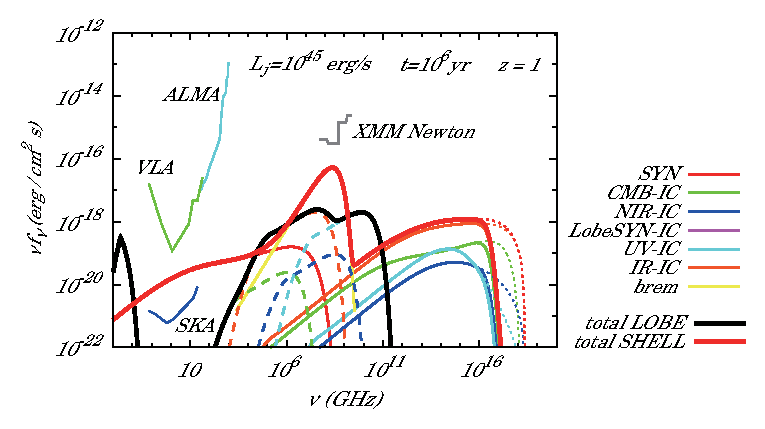
\includegraphics[width=0.8\textwidth]{transients/transients.s3.agn.fig1.eps}
		\caption{ジェットの放出が停止した (死んだ) 電波銀河に付随するローブ (黒実線) 及びシェル (赤実線) のスペクトル。
		電波銀河の年齢を$10^6$年、ジェットが活動を停止するまでの継続時間を$10^5$年と仮定し、また赤方偏移を$z=1$としている (Ito et al., 2015, submitted to ApJ)。}
		\label{fig:transients.s3.agn.fig1}
\end{figure}%

%% Author: 端山和大

\subsection{重力波--電波マルチメッセンジャー観測} \label{transients.s3.gw}
近年、オーストラリアのParkes電波望遠鏡によりFRBと呼ばれる継続時間数msの突発的な電波天体が相次いで観測され (\Secref{transients.s1.frb})、日本でも \Figref{fig:transients.s3.gw.nasu}の那須電波観測所によって、数分から数日といったFRBより長いタイムスケールの突発天体 (WJN電波トランジェント; \Secref{transients.s3.unknowns}) が観測されている。
こういった電波帯域における突発天体は未だ対応天体が発見されておらず、その起源の解明はこれからの電波天文学にとって重要なテーマの一つである。
\begin{figure}
	\centering
	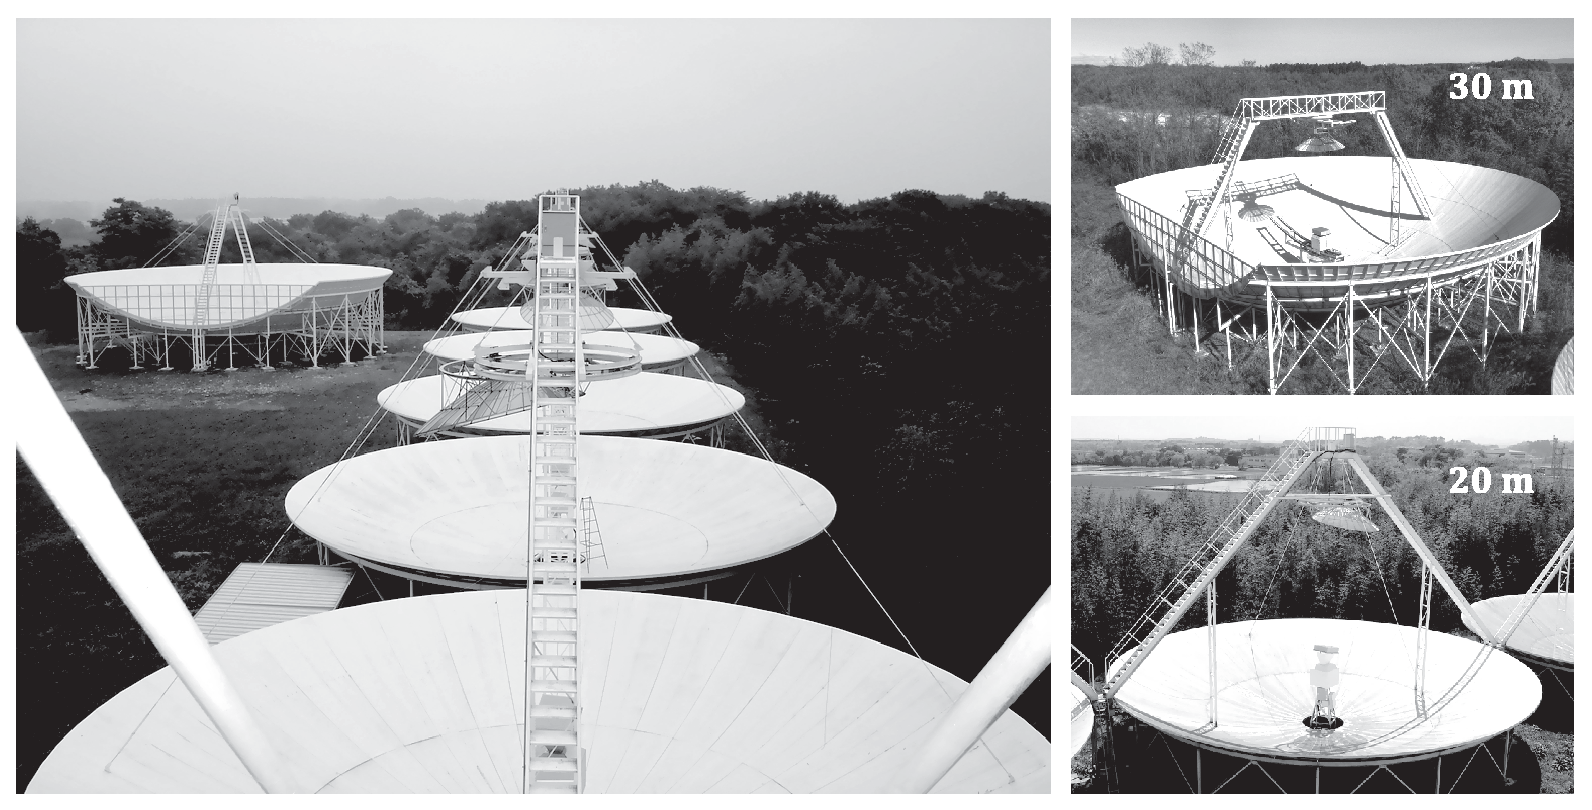
\includegraphics[width=1\textwidth]{transients/transients.s3.gw.nasu.eps}
	\caption{那須電波観測所。口径 20~m の電波望遠鏡8基、30~mの電波望遠鏡1基をもつ。}
	\label{fig:transients.s3.gw.nasu}
\end{figure}%

こうした突発天体は、そのエネルギーとタイムスケールから、重力波を伴うような天体爆発現象である可能性が示唆されている。
FRBのモデルとしては、重力波天体として最有力候補の一つである中性子連星合体時に起きるシンクロトロン放射\citep{2013PASJ...65L..12T}があり、またWJNイベントのモデルとしては、中性子星連星合体後に起きる電波アフターグローモデルが考えられる \citep{2011Natur.478...82N}。
さらに連星合体の際は、\Secref{transients.s1.grb}で述べたようにshort GRBも付随することが予想される。
そこで重力波と電波を中心とした、「マルチメッセンジャー観測」と呼ばれる多粒子・多波長による連携観測により、天体現象の多角的理解を目指す観測体制の構築が重要になる \citep{2012IAUS..285..331H}。

FRBの本来のイベントレートはおよそ$2 \times 10^4~\text{Gpc}^{-3}~\text{yr}^{-1}$ と見積もられており、現在建設中の重力波望遠鏡が見通せる、地球から$200~\text{Mpc}$ 以内で起こりうるFRBは、年間$160$ 個程度と考えられる。
このイベントレートは現在見積もられている連星中性子星合体のイベントレートの誤差範囲内にある。
もしFRBの起源が重力波天体であり、かつすべて検出できるならば、2020年には年間$160$程度の重力波--FRB同時観測が行われ、統計的な議論もできるようになると考えられる。
こうした突発天体を捉えるためには広い視野で長期間観測して天球上を走査することが最も有効になる。
SKAで採用が検討されている Phased Array Feed (PAF) は $18~\text{deg}^2$ という広い視野を持ち、\skasur{1} プログラムでは1年間で$550$時間、走査領域にして$10,000~\text{deg}^2$をカバーすることが予定されており、非常に有望な重力波マルチメッセンジャー観測体制を担う望遠鏡である。
さらにSKAでAdvanced Instrumentation Program (AIP) となっているMid-frequency Aperture Array (MAA) は、$200~\sqdeg$という驚異的な広視野を持ち、その実装は電波天文学のみならず重力波天文学にとっても極めて重要である。

\subsection{FRBの偏波の可能性と宇宙磁場} \label{transients.s3.frb.magnetism}

今現在までに、FRBに有意な直線偏波は検出されていない\footnote{円偏波は1例観測された \citep{2015MNRAS.447..246P}。}。それがFRB現象に普遍的な現象なのか、または偶然なのか、その判断をするにはまだ発見数はあまりにも少ない。もしFRBに直線偏波が含まれるなら、ファラデー効果の分散測度 (DM) に加えてファラデー回転測度 (RM) も計測できる可能性がある。そうなった場合、密度重みつき視線平均磁場強度$\langle B_\parallel \rangle $をDMとRMの定義から
\begin{equation}
\langle B_\parallel \rangle =\frac{{\it RM}}{{\it DM}}
\end{equation}
という式で簡単に求めることができる。FRBが系外起源であるならば、この磁場強度の推定には銀河間磁場の情報を含む。電波銀河など系外偏波源を使ってRMを測る場合はDMは測らない (測れない) ため、このように単一観測から磁場強度まで推定できるのは画期的なことである。一つの視線だけでは系内と系外の寄与を切り分けるのは難しいかもしれないが、沢山の観測で統計を高めることで、銀経・銀緯に依存しないが赤方偏移に依存するような「超過成分」として銀河間磁場の寄与が議論できるかもしれない。SKAのサーベイ能力は、そのような統計的な議論をはじめて可能にするだろう。具体的で確実な調査の方法論を理論的に検討していくことも不可欠であるが、日本は銀河間磁場の調査で世界をリードしているので\citep{2014PASJ...66...65A,2014ApJ...790..123A}、日本のSKAサイエンスの特色の一つとできるだろう。FRBが銀河間磁場を探る新しい方法となるかもしれない。
%% Author: 青木貴弘
\subsection{未知の突発天体の探査} \label{transients.s3.unknowns}
{ %% Localize settings
\newcommand{\suffix}[2]{^{> #1 \, \text{mJy}} _{#2 \, \text{GHz}}}
\newcommand{\ntt}{那須 20~m 電波望遠鏡}
\newcommand{\WJN}{WJN J1443+3439}
\newcommand{\FDR}{{\it FDR}}
\newcommand{\siglevel}{\mbox{$10^{-5}$}~}
\newcommand{\ssd}{天球面密度}

%% Body
%%
%% ss1
%%
\subsubsection{従来の探査結果}
他の波長域で対応天体が見つからないような、未知の突発天体の探査が何度か行われてきている。
例えば\citet{2002ApJ...576..923L}は orphan GRB afterglow をカタログ比較によって探査し、9つの候補天体を発見した。
その後、追観測やデータの再解析によって8つが偽陽性検出であることが判明し、1つについては電波のみを放射しているII型超新星とわかりVLA~121550.2+130654 と命名された \citep{2006ApJ...639..331G,2010ApJ...711..517O}。

それ以降、未知の突発天体探査が活発化し、それらの探査結果を図示したものが\Figref{fig:transients.s3.unknowns.rate}である。
図中の各プロットは脚注に示す文献に基づいている\footnote{
\Figref{fig:transients.s3.unknowns.rate}の各プロットは次の文献をもとにしている: \citealt{2007ApJ...666..346B} (Bow07 2-month/single), \citealt{2010ApJ...725.1792B} (Bow10a/b), \citealt{2011ApJ...740...65O} (Ofe11), \citealt{2012AJ....143...96J} (Jae12), \citealt{2006ApJ...639..331G} (Gal06), \citealt{2011MNRAS.412..634B} (Ban11), \citealt{2010ApJ...719...45C} (Cro10),  \citealt{2011ApJ...728L..14B} (Bow11a/b), \citealt{2014ApJ...781...10A} (Aok14), \citealt{2010AJ....140.1995L} (Laz10)。
いくつかのプロットは\citet{2011MNRAS.415....2B}, \citet{2012ApJ...747...70F}にまとめられている。
}。
\Figref{fig:transients.s3.unknowns.rate}の横軸は観測感度、つまり最小検出フラックス密度$S$を表し、縦軸は天球上の単位面積を観測したときに、フラックス密度が$S$を超える未知天体を発見できる個数、つまり天球面上の個数密度$\varSigma (>S)$を表す。
この天球面上の個数密度 (sky-surface density) はスナップショットレート (snapshot rate) とも呼ばれ、イメージング観測の結果として導くことができる発見確率の指標であり、この量をイベントレートに換算することができる。
\begin{figure}
	\centering
	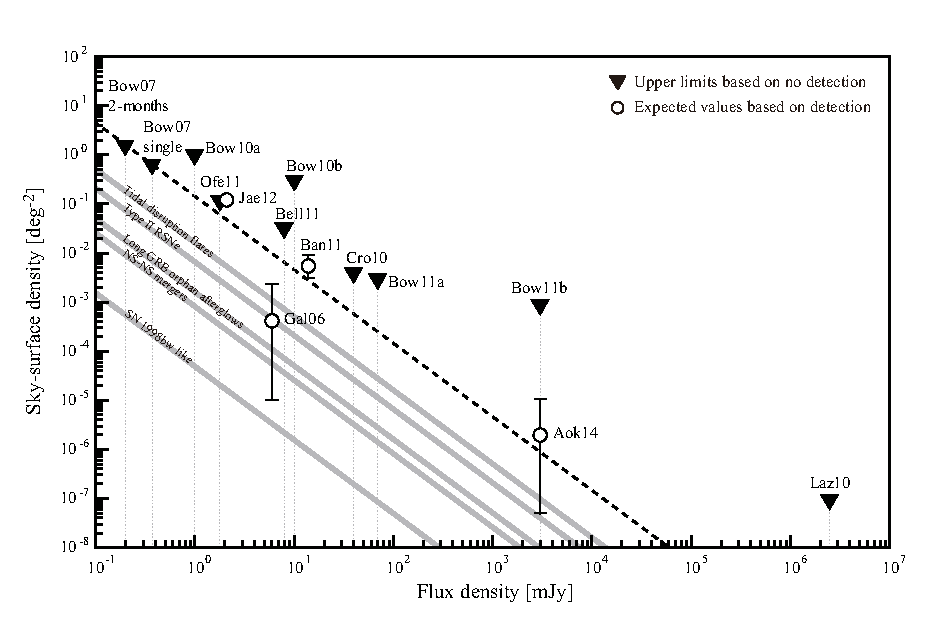
\includegraphics[width=1\textwidth]{transients/transients.s3.unknowns.rate.eps}
	\caption{未知の突発天体に対する、天球面上の個数密度$\varSigma (>S)$ とフラックス密度 $S$ の関係 \citep{2014ApJ...781...10A}。
	ただし観測周波数は考慮していない。
	三角形のプロットは突発天体が発見されなかった探査結果を示し、円形のプロットはいくつかの発見があった探査結果を示す。
	灰色の太線は\citet{2012ApJ...747...70F}によって推定された、既知天体の個数密度を表している。}
	\label{fig:transients.s3.unknowns.rate}
\end{figure}%

これらの探査によって、いくつかの候補天体が発見されてきているが、その起源のみならず発見の真偽についても確証は得られていない。
この検証のためには、従来の観測装置の性能では多くの観測時間が必要となり現実的ではなく、SKAによる広視野・高感度な探査観測が必要となる。
そこで、これらの検証のためにSKAに必要な性能を、早稲田大学の那須電波観測所による探査結果を例にして提案する。

%%
%% ss2
%%
\subsubsection{従来の探査結果の検証}
\paragraph{検証の方法}
\Figref{fig:transients.s3.unknowns.rate}の Aok14 というプロットは、那須電波観測所 (\Figref{fig:transients.s3.gw.nasu}) で行った突発天体の探査結果を示している。
その探査では、1日程度の継続時間をもつ起源不明の突発天体を発見し、\WJN と命名した \citep{2007ApJ...657L..37N}。
この発見から、周波数1.42 GHzにおいてフラックス密度3000~mJy以上を持つ未知の突発天体の個数密度は、$\varSigma \suffix{3000}{1.42} = 2^{+9}_{-1.9} \times 10^{-6}~\persqdeg$ と見積もられる\footnote{
\citet{2010ApJ...711..517O}の定義に従えばイベントレート $\mathfrak{R}$ は個数密度$\varSigma$と光度変動の継続時間$W$を用いて$\mathfrak{R} = \varSigma / W$で与えられ、那須電波観測所で発見されたWJNイベントに対しては$%
	\mathfrak{R}\suffix{3000}{1.42} = 7^{+33}_{-7} \times 10^{-4}(W/\text{day})^{-1} \persqdeg \peryr 
	= 30^{+136}_{-28} (W/\text{day})^{-1} \persky \peryr%
$
を得る。
単位 sky は全天$4\pi~\text{sr}$として定義した。
}。
したがって任意のフラックス密度$S$における個数密度は
\begin{equation}
	\varSigma^{>S}_{\text{1.42~GHz}} = 0.3~\persqdeg \times \left(  S/\text{mJy} \right)^{-3/2}
	\label{eq:transients.s3.unknowns.nasu-dens}
\end{equation}
で推定できる。
この観測結果の正当性は、広い面積を高い感度で探査することによって検証が可能である。
\Eqref{eq:transients.s3.unknowns.nasu-dens}という結果を検証するために必要な、探査観測の感度$S$と掃天面積$\varOmega$の関係は、統計的な議論によって\footnote{
突発現象の生起個数はポアソン過程であるから事象の生起間隔 $\varOmega$ は指数分布となり、突発天体を発見できる確率は$P(\varOmega)=1-\e^{-\varSigma \varOmega}$で与えられる。
このとき95\% 以上の確率で少なくとも一つの天体を発見するために必要な掃天面積$\varOmega$ は$P(\varOmega) \leq 95\%$で与えられる。
}
\begin{equation}
	\varOmega / \sqdeg > 10 \times \left( S/\text{mJy} \right)^{+3/2}
	\label{eq:transients.s3.unknowns.survey-config}
\end{equation}
で与えられる \citep{2014ApJ...781...10A}。
この関係を満たす観測を行えば95\% の確率で同様の突発天体を検出できるはずであり、もし検出できなければ\Eqref{eq:transients.s3.unknowns.nasu-dens}という観測結果は棄却されうることになる。
このようにして那須電波観測所による探査結果のみならず、\Figref{fig:transients.s3.unknowns.rate}に示す従来の結果の多くを検証することができる。

\paragraph{検証のためのSKAへの要求}
SKA Phase 1 を用いて\Eqref{eq:transients.s3.unknowns.survey-config}を満たす観測を行えば、従来の探査結果を検証することができる。
%装置要求をするにあたり、既にデザインされている性能パラメーターのいくつかを固定し、アンテナ台数と受信機冷却に関係するパラメーター、実効開口面積$A_\text{e}$とシステム雑音温度$T_\text{sys}$を不定として、感度パラメーター$A_\text{e}/T_\text{sys}$に対する要求を述べる。
GHz帯域で行われてきた従来の探査を検証するという観点からは、必要になるのは\skamid{} または \skasur{} のアンテナであり、突発天体探査で最も重要な要素は視野の広さであるから、\skasur{}が最も適したアンテナといえる。
そこで主に\skasur{1}アンテナの基本デザインをもとに、検証に必要な system equivalent flux density (SEFD) を考える。

\skasur{1} アンテナには phased array feed (PAF) とよばれるフィードが搭載される予定であり、既存のASKAPの周波数帯域を考えると、SKA1で最初に実装するのは PAF Band~2 (周波数650--1670~MHz、視野 $18~\sqdeg$) が妥当だろう。
また観測可能な帯域幅は片偏波あたり最大500~MHzとされている。
最小検出フラックスを$S_\text{min}=\text{SEFD}_\text{array}/(\eta_\text{s}\sqrt{\varDelta \nu \ \tau})$とし検出閾値を$S=7S_\text{min}$とすると、\Eqref{eq:transients.s3.unknowns.survey-config}を満たすようなSEFDは
\begin{align}
	\text{SEFD}_\text{array} 
	< 260~\text{Jy} \times \left( \frac{\varOmega}{18~\sqdeg} \right)^{2/3}
		\cdot \frac{\eta_\text{s}}{0.9} \cdot 
		\sqrt{\frac{\varDelta \nu}{500~\text{MHz}} \cdot \frac{\tau}{1~\text{hour}}}
	%&= 15~\text{Jy} \cdot \left( \frac{\varOmega}{18~\sqdeg} \right)^{2/3}
	%	\cdot \frac{\eta_\text{s}}{0.9} \cdot 
	%	\sqrt{\frac{\varDelta \nu}{100~\text{MHz}} \cdot \frac{\tau}{1~\text{min}}}
		\label{eq:transients.s3.unknowns.sefd}
\end{align}
となる\footnote{\Eqref{eq:transients.s3.unknowns.sefd}は\skasur{1}の性能を単位としているが、当然\skamid{1}への要求検討にも使用できる。}。
ここで$\eta_\text{s}$はシステム効率、$\varDelta \nu$は観測帯域幅、$\tau$は積分時間を表す。
SKAの基本的な性能はおおよそ固まっているため、例えば建設するべきアンテナの台数に着目すると、現状の単一鏡のデザイン $\text{SEFD}_\text{dish}=586~\text{Jy}$ が実現するとすれば、上記の検証観測をするには{\ 感度のみの観点からは}3台で事足りる\footnote{$\text{SEFD}_\text{array} \simeq \text{SEFD}_\text{dish}/m$, $m=\text{アンテナの台数}$。}。
ただしもちろんこの見積もりは、光度変動のタイムスケールが1時間以上の突発天体に対するものである。

\WJN の継続時間は4分以上3日以内としか制限されておらず、またGCRT J1745-3009 のように数分スケールの電波変動を起こす天体を観測しようとすると (\Secref{transients.s1.unknowns})、上記の見積もりではその観測は実現できない。
また500~MHzという帯域幅は使用可能な上限値であり、実際の観測ではより狭帯域に制限されることもありうる。
そのような状況を考え、帯域幅100~MHzを積分時間1~minで観測することを考えると$\text{SEFD}_\text{array}=15~\text{Jy}$が必要になり、その場合アンテナは40台必要になる。
ただし\skasur{1} の計画では60台のアンテナを建設予定であり\footnote{\skasur{1}アンテナ60台、ASKAPアンテナ36台で計96台のアンテナを運用することも計画されているが、本節の見積もりにASKAPアンテナは含めていない。}、$\text{SEFD}_\text{array}=10~\text{Jy}$を得られるから、上記の検証観測は十分に実施可能である。
積分時間が1~minという観測では$u$--$v$平面の埋まりが悪いが、\Figref{fig:transients.phasespace}の中央付近の空白領域を埋めることにつながり、未知の突発天体の探査には重要な時間分解能である。

\subsubsection{未知の探査}

%既に理論的に存在することは知られているが実際に観測されたことはない、あるいは数例の観測例はあるものの確証が得られていない天体、つまり\Secref{transients.s2.wilkinson}で述べた「既知の未知 (known unknowns)」の探査をすることが、今後の電波天文学にとって重要である。
%この点について、SKAは他の電波望遠鏡に比べて極めて強いアドバンテージを持っており、その探査をすることは宇宙科学にブレイクスルーを起こせる数少ない手段の一つである。

未知の天体の例としては、\Secref{transients.s1}や\Figref{fig:transients.s3.unknowns.rate}にも示した潮汐崩壊現象や orphan GRB afterglow などがあり、前者は Swift J1644+57 という観測例があるが詳細はわかっておらず、後者は観測例もない。
これらを能動的に探査することがSKAには求められ、実際に発見するために必要な性能をSKAに持たせなければならない。
そこでここでは、\skasur{1}による探査と発見のための要求性能を考える。


\citet{2012ApJ...747...70F}の見積もりによれば\Figref{fig:transients.s3.unknowns.rate}の斜線に示したように、可視光放射がないII型電波超新星 \citep{2006ApJ...639..331G} の個数密度は$\varSigma^{>S} = 6.6\times 10^{-3}~\persqdeg \times (S/\text{mJy})^{-3/2}$である。
このレートを単位にして、電波帯域における突発天体を95\% 以上の確率で発見するために必要な観測は、
\begin{align}
	\biggl( \frac{\text{SEFD}_\text{array}}{10~\text{Jy}} \biggr)^{-2}
	\biggl( \frac{\varOmega}{18~\sqdeg} \biggr)^{4/3} 
	\biggl( \frac{\eta_\text{s}}{0.9} \biggr)^2 \cdot 
	\frac{\varDelta \nu}{500~\text{MHz}} \cdot \frac{\tau}{6~\text{hour}}
	> 0.041
	\label{eq:transients.s3.unknowns.SNII}
\end{align}
という関係を満たすような観測設定をする必要がある\footnote{$\text{SEFD}_\text{dish} = 586~\text{Jy}$のSKAアンテナ60台で干渉計を構成すると、$\text{SEFD}_\text{array} = 10~\text{Jy}$を得る。}。
したがって、例えば15分程度の観測をするだけで、従来数々の電波望遠鏡を駆使してようやく発見した、可視光対応天体のないII型超新星を95\% の確率で発見できるということである。

しかし一方で、Ic型極超新星SN 1998bw (GRB 980425) と同様の突発天体を探査しようとすると、個数密度が$\varSigma^{>S} = 4.9\times 10^{-5}~\persqdeg \times (S/\text{mJy})^{-3/2}$でありイベントレートが低すぎるため、電波帯域だけで探査しようとすると約180時間の観測時間が必要となる。
これを実現するには、約1か月間に渡って受信機性能を安定化させ、かつデータ較正をするシステムが必要になるだろう。

\subsubsection{まとめ}

従来さまざまな電波望遠鏡を用いて、未知の突発天体が探査されてきているが、視野の広さと感度の高さが両立した観測は難しく、効果的な探査は行われてこなかった。
SKAはこの現状を打破し、とりわけ\skasur{} は広い視野、高い感度、高い空間分解能を同時に実現し、突発天体研究にとって強力なツールとなるだろう。
単に従来の探査結果を検証するだけならば、\skasur{1} アンテナの台数は5台もあれば可能だが、それでは理論的に予測されているが実観測例のない orphan GRB afterglow や Ia 型超新星の研究を行うことができない。
したがって現状のデザインを実現することが重要である。
そしてその探査が実現すれば、まだ観測例のない突発天体も容易に発見できると見積もられる。




} %% End of localization

%%
\subsection{突発天体研究のためのSKAへの要求} \label{transients.s3.requirements}
%%

SKAは既にデザインがおおよそ決まっており、その装置性能や運用体制に対して修正を要求することは難しい。
そのことを踏まえて本節では、現状のデザインでどの程度のサイエンスを進められるか、あるいは最低限必要な性能は何かという点について主に言及してきた。
ここではそれらについて再度簡単にまとめる。

\subsubsection{アンテナの選択}
突発天体研究の進め方は二通りあり、(1) 他波長で発見された突発天体を追観測するという方法と、(2) 新たな突発天体を求めて主体的に探査するという方法がある。
どちらの方法も重要であり、(1) では従来の望遠鏡ではなしえない感度によって、起源天体の物理の解明をめざし、(2) では、理論予測はされていてもまだ観測されていないような天体を発見し、さらには人類がまだ予想すらしていないような未知の発見を生む可能性が高い。
そして強いて言うならば、(1) は主に\skamid{}によって実施され、(2) は\skasur{}によって実施される。
また\skalow{}は装置の特色上 (1) と (2) 両方に注力できる。

\skamidsur{} はどちらも主鏡は同じものを使用するが、そのフィードや受信機系は異なり、\skamid{}は広帯域、高感度、高分解能に、\skasur{}は広い視野による探査速度に長けている。
日本の既存望遠鏡との連携という観点からは、時差のほとんどないオーストラリアに建設される\skasur{}が突発天体探査と追観測には有利といえる\footnote{ただし北半球の日本と南半球のオーストラリアでは観測範囲が重ならないことも多い。}。
現状の突発天体研究においては、起源がわかっていないものなどは300~MHzなどの低周波帯 (e.g., GCRT)、あるいは1.4~GHz帯に多く見つかっている (e.g., FRB)。
一方で超新星などの場合5~GHz帯での観測がよく行われており、\skalowmidsur{} の全てが突発天体研究にとっては重要な装置である。
しかし現状の日本の突発天体コミュニティでは、主に\skamidsur{} を用いたサイエンスの提案が多いため、現時点では主にそれらに絞って装置性能を考える。

\subsubsection{装置要求}
以上のことを踏まえて、以下で各観測パラメータについて簡単にまとめる。

\paragraph{周波数範囲}
従来発見されてきた突発天体は数十MHzという低周波からGHz帯まで幅広く発見されてきており、特別な周波数というものはない。
ただしFRBやパルサー観測では主に1.4~GHz帯で強度が強いため観測しやすく、またその周波数帯は中性水素輝線の観測で重要であるから、Lバンドを観測できる受信機の実装を最優先すべきである。
\citet{2011Natur.478...82N}によれば、中性子星連星合体で重力波とともに1.4~GHzでピークをもつ電波が放射されるので、Lバンド受信機の実装は重力波天文学においても重要である。
また超新星やGRBの観測ではより高周波帯を観測する必要があり、Cバンド受信機などの実装も急ぐべきである。

\paragraph{感度}
感度は高ければ高いだけ良い。
例えば超新星の検出数と感度との関係は\Secref{transients.s2}の原論文に書かれており、また未知の突発天体の探査に必要な感度は、例えば\Eqref{eq:transients.s3.unknowns.SNII}を満たす範囲で、コストに見合う性能を追求すればよい。

\paragraph{時間分解能}
突発天体探査においては、時間分解能の多様性が極めて重要な要素である。
これまで発見されてきた突発天体は、Crab nanoshots のようなナノ秒スケールの変動や、FRBや普通のパルサーのようなミリ秒程度の変動、またGCRTイベントのような数分スケールの変動からWJNイベントのような数時間、数日程度の変動、さらにGRB残光のような数か月、数年という変動など、あらゆる時間領域に渡っている。
したがって、それらを網羅できるような時間分解観測が必要である。
このうち、パルス観測はコンピュータによる計算コストは高いが、観測自体は容易であり、また数日以上続くような長時間変動の場合も、通常の干渉計観測を行えばよく容易といえる。
おそらく観測自体がやや難しい (面倒な) のは変動のタイムスケールが数分程度の現象であり、感度と空間分解能をいかに維持して数分スケールの変動を追うかが課題になるだろう。

\paragraph{偏波}
偏波情報は、突発現象の放射機構解明などに必須であり、その受信系は必ず実装すべきである。
また\Secref{transients.s3.frb.magnetism}に記したように、FRBを用いて銀河間磁場を解明できる可能性もある。

\subsubsection{まとめ}
SKAデザインは基本的には決められており、またその既存デザインで、日本コミュニティの期待する成果は十分に出せると見積もっている。
未知天体の探査については、その最低限の要求は\Eqref{eq:transients.s3.unknowns.SNII}で与えており、その要求を満たせば多くの超新星などが発見され、それらの研究において大きなブレイクスルーとなる。


\begin{thebibliography}{99}
\addcontentsline{toc}{section}{参考文献}
\markboth{参考文献}{参考文献}
\begin{multicols}{2}{\footnotesize
\expandafter\ifx\csname natexlab\endcsname\relax\def\natexlab#1{#1}\fi

\bibitem[{{Ackermann} {et~al.}(2013){Ackermann}, {Ajello}, {Allafort},
  {Baldini}, {Ballet}, {Barbiellini}, {Baring}, {Bastieri}, {Bechtol},
  {Bellazzini}, {Blandford}, {Bloom}, {Bonamente}, {Borgland}, {Bottacini},
  {Brandt}, {Bregeon}, {Brigida}, {Bruel}, {Buehler}, {Busetto}, {Buson},
  {Caliandro}, {Cameron}, {Caraveo}, {Casandjian}, {Cecchi}, {{\c C}elik},
  {Charles}, {Chaty}, {Chaves}, {Chekhtman}, {Cheung}, {Chiang}, {Chiaro},
  {Cillis}, {Ciprini}, {Claus}, {Cohen-Tanugi}, {Cominsky}, {Conrad}, {Corbel},
  {Cutini}, {D'Ammando}, {de Angelis}, {de Palma}, {Dermer}, {do Couto e
  Silva}, {Drell}, {Drlica-Wagner}, {Falletti}, {Favuzzi}, {Ferrara},
  {Franckowiak}, {Fukazawa}, {Funk}, {Fusco}, {Gargano}, {Germani},
  {Giglietto}, {Giommi}, {Giordano}, {Giroletti}, {Glanzman}, {Godfrey},
  {Grenier}, {Grondin}, {Grove}, {Guiriec}, {Hadasch}, {Hanabata}, {Harding},
  {Hayashida}, {Hayashi}, {Hays}, {Hewitt}, {Hill}, {Hughes}, {Jackson},
  {Jogler}, {J{\'o}hannesson}, {Johnson}, {Kamae}, {Kataoka}, {Katsuta},
  {Kn{\"o}dlseder}, {Kuss}, {Lande}, {Larsson}, {Latronico}, {Lemoine-Goumard},
  {Longo}, {Loparco}, {Lovellette}, {Lubrano}, {Madejski}, {Massaro}, {Mayer},
  {Mazziotta}, {McEnery}, {Mehault}, {Michelson}, {Mignani}, {Mitthumsiri},
  {Mizuno}, {Moiseev}, {Monzani}, {Morselli}, {Moskalenko}, {Murgia},
  {Nakamori}, {Nemmen}, {Nuss}, {Ohno}, {Ohsugi}, {Omodei}, {Orienti},
  {Orlando}, {Ormes}, {Paneque}, {Perkins}, {Pesce-Rollins}, {Piron}, {Pivato},
  {Rain{\`o}}, {Rando}, {Razzano}, {Razzaque}, {Reimer}, {Reimer}, {Ritz},
  {Romoli}, {S{\'a}nchez-Conde}, {Schulz}, {Sgr{\`o}}, {Simeon}, {Siskind},
  {Smith}, {Spandre}, {Spinelli}, {Stecker}, {Strong}, {Suson}, {Tajima},
  {Takahashi}, {Takahashi}, {Tanaka}, {Thayer}, {Thayer}, {Thompson},
  {Thorsett}, {Tibaldo}, {Tibolla}, {Tinivella}, {Troja}, {Uchiyama}, {Usher},
  {Vandenbroucke}, {Vasileiou}, {Vianello}, {Vitale}, {Waite}, {Werner},
  {Winer}, {Wood}, {Wood}, {Yamazaki}, {Yang}, \&
  {Zimmer}}]{2013Sci...339..807A}
{Ackermann}, M., {et~al.} 2013, Science, 339, 807

\bibitem[{{Akahori} {et~al.}(2014{\natexlab{a}}){Akahori}, {Gaensler}, \&
  {Ryu}}]{2014ApJ...790..123A}
{Akahori}, T., {Gaensler}, B.~M., \& {Ryu}, D. 2014{\natexlab{a}}, \apj, 790,
  123

\bibitem[{{Akahori} {et~al.}(2014{\natexlab{b}}){Akahori}, {Kumazaki},
  {Takahashi}, \& {Ryu}}]{2014PASJ...66...65A}
{Akahori}, T., {Kumazaki}, K., {Takahashi}, K., \& {Ryu}, D.
  2014{\natexlab{b}}, \pasj, 66, 65

\bibitem[{{Anderson} {et~al.}(2014){Anderson}, {van der Horst}, {Staley},
  {Fender}, {Wijers}, {Scaife}, {Rumsey}, {Titterington}, {Rowlinson}, \&
  {Saunders}}]{2014MNRAS.440.2059A}
{Anderson}, G.~E., {et~al.} 2014, \mnras, 440, 2059

\bibitem[{{Aoki} {et~al.}(2014){Aoki}, {Tanaka}, {Niinuma}, {Takefuji}, {Kida},
  {Nakao}, {Nomura}, {Sugisawa}, \& {Daishido}}]{2014ApJ...781...10A}
{Aoki}, T., {et~al.} 2014, \apj, 781, 10

\bibitem[{{Bannister} {et~al.}(2011){Bannister}, {Murphy}, {Gaensler},
  {Hunstead}, \& {Chatterjee}}]{2011MNRAS.412..634B}
{Bannister}, K.~W., {Murphy}, T., {Gaensler}, B.~M., {Hunstead}, R.~W., \&
  {Chatterjee}, S. 2011, \mnras, 412, 634

\bibitem[{{Bell} {et~al.}(2011){Bell}, {Fender}, {Swinbank}, {Miller-Jones},
  {Law}, {Scheers}, {Spreeuw}, {Wise}, {Stappers}, {Wijers}, {Hessels}, \&
  {Masters}}]{2011MNRAS.415....2B}
{Bell}, M.~E., {et~al.} 2011, \mnras, 415, 2

\bibitem[{{Bloom} {et~al.}(2011){Bloom}, {Giannios}, {Metzger}, {Cenko},
  {Perley}, {Butler}, {Tanvir}, {Levan}, {O'Brien}, {Strubbe}, {De Colle},
  {Ramirez-Ruiz}, {Lee}, {Nayakshin}, {Quataert}, {King}, {Cucchiara},
  {Guillochon}, {Bower}, {Fruchter}, {Morgan}, \& {van der
  Horst}}]{2011Sci...333..203B}
{Bloom}, J.~S., {et~al.} 2011, Science, 333, 203

\bibitem[{{Bower} \& {Saul}(2011)}]{2011ApJ...728L..14B}
{Bower}, G.~C., \& {Saul}, D. 2011, \apjl, 728, L14

\bibitem[{{Bower} {et~al.}(2007){Bower}, {Saul}, {Bloom}, {Bolatto},
  {Filippenko}, {Foley}, \& {Perley}}]{2007ApJ...666..346B}
{Bower}, G.~C., {Saul}, D., {Bloom}, J.~S., {Bolatto}, A., {Filippenko}, A.~V.,
  {Foley}, R.~J., \& {Perley}, D. 2007, \apj, 666, 346

\bibitem[{{Bower} {et~al.}(2010){Bower}, {Croft}, {Keating}, {Whysong},
  {Ackermann}, {Atkinson}, {Backer}, {Backus}, {Barott}, {Bauermeister},
  {Blitz}, {Bock}, {Bradford}, {Cheng}, {Cork}, {Davis}, {DeBoer}, {Dexter},
  {Dreher}, {Engargiola}, {Fields}, {Fleming}, {Forster}, {Gutierrez-Kraybill},
  {Harp}, {Heiles}, {Helfer}, {Hull}, {Jordan}, {Jorgensen}, {Kilsdonk}, {Law},
  {van Leeuwen}, {Lugten}, {MacMahon}, {McMahon}, {Milgrome}, {Pierson},
  {Randall}, {Ross}, {Shostak}, {Siemion}, {Smolek}, {Tarter}, {Thornton},
  {Urry}, {Vitouchkine}, {Wadefalk}, {Weinreb}, {Welch}, {Werthimer},
  {Williams}, \& {Wright}}]{2010ApJ...725.1792B}
{Bower}, G.~C., {et~al.} 2010, \apj, 725, 1792

\bibitem[{{Burke-Spolaor} {et~al.}(2011){Burke-Spolaor}, {Bailes}, {Ekers},
  {Macquart}, \& {Crawford}}]{2011ApJ...727...18B}
{Burke-Spolaor}, S., {Bailes}, M., {Ekers}, R., {Macquart}, J.-P., \&
  {Crawford}, III, F. 2011, \apj, 727, 18

\bibitem[{{Burlon} {et~al.}(2015){Burlon}, {Ghirlanda}, {van der Horst},
  {Murphy}, {Wijers}, {Gaensler}, {Ghisellini}, \&
  {Prandoni}}]{2015arXiv150104629B}
{Burlon}, D., {Ghirlanda}, G., {van der Horst}, A., {Murphy}, T., {Wijers}, R.,
  {Gaensler}, B., {Ghisellini}, G., \& {Prandoni}, I. 2015, ArXiv e-prints

\bibitem[{{Bykov} {et~al.}(2000){Bykov}, {Chevalier}, {Ellison}, \&
  {Uvarov}}]{2000ApJ...538..203B}
{Bykov}, A.~M., {Chevalier}, R.~A., {Ellison}, D.~C., \& {Uvarov}, Y.~A. 2000,
  \apj, 538, 203

\bibitem[{{Camilo} {et~al.}(2006){Camilo}, {Ransom}, {Halpern}, {Reynolds},
  {Helfand}, {Zimmerman}, \& {Sarkissian}}]{2006Natur.442..892C}
{Camilo}, F., {Ransom}, S.~M., {Halpern}, J.~P., {Reynolds}, J., {Helfand},
  D.~J., {Zimmerman}, N., \& {Sarkissian}, J. 2006, \nat, 442, 892

\bibitem[{{Camilo} {et~al.}(2008){Camilo}, {Reynolds}, {Johnston}, {Halpern},
  \& {Ransom}}]{2008ApJ...679..681C}
{Camilo}, F., {Reynolds}, J., {Johnston}, S., {Halpern}, J.~P., \& {Ransom},
  S.~M. 2008, \apj, 679, 681

\bibitem[{{Caprioli} \& {Spitkovsky}(2014)}]{2014ApJ...783...91C}
{Caprioli}, D., \& {Spitkovsky}, A. 2014, \apj, 783, 91

\bibitem[{{Castelletti} {et~al.}(2007){Castelletti}, {Dubner}, {Brogan}, \&
  {Kassim}}]{2007A&A...471..537C}
{Castelletti}, G., {Dubner}, G., {Brogan}, C., \& {Kassim}, N.~E. 2007, \aap,
  471, 537

\bibitem[{{Chandra} {et~al.}(2012){Chandra}, {Chevalier}, {Chugai}, {Fransson},
  {Irwin}, {Soderberg}, {Chakraborti}, \& {Immler}}]{2012ApJ...755..110C}
{Chandra}, P., {Chevalier}, R.~A., {Chugai}, N., {Fransson}, C., {Irwin},
  C.~M., {Soderberg}, A.~M., {Chakraborti}, S., \& {Immler}, S. 2012, \apj,
  755, 110

\bibitem[{{Chandra} \& {Frail}(2012)}]{2012ApJ...746..156C}
{Chandra}, P., \& {Frail}, D.~A. 2012, \apj, 746, 156

\bibitem[{{Chevalier}(1998)}]{1998ApJ...499..810C}
{Chevalier}, R.~A. 1998, \apj, 499, 810

\bibitem[{{Chomiuk} {et~al.}(2012){Chomiuk}, {Soderberg}, {Moe}, {Chevalier},
  {Rupen}, {Badenes}, {Margutti}, {Fransson}, {Fong}, \&
  {Dittmann}}]{2012ApJ...750..164C}
{Chomiuk}, L., {et~al.} 2012, \apj, 750, 164

\bibitem[{{Croft} {et~al.}(2010){Croft}, {Bower}, {Ackermann}, {Atkinson},
  {Backer}, {Backus}, {Barott}, {Bauermeister}, {Blitz}, {Bock}, {Bradford},
  {Cheng}, {Cork}, {Davis}, {DeBoer}, {Dexter}, {Dreher}, {Engargiola},
  {Fields}, {Fleming}, {Forster}, {Gutierrez-Kraybill}, {Harp}, {Helfer},
  {Hull}, {Jordan}, {Jorgensen}, {Keating}, {Kilsdonk}, {Law}, {van Leeuwen},
  {Lugten}, {MacMahon}, {McMahon}, {Milgrome}, {Pierson}, {Randall}, {Ross},
  {Shostak}, {Siemion}, {Smolek}, {Tarter}, {Thornton}, {Urry}, {Vitouchkine},
  {Wadefalk}, {Welch}, {Werthimer}, {Whysong}, {Williams}, \&
  {Wright}}]{2010ApJ...719...45C}
{Croft}, S., {et~al.} 2010, \apj, 719, 45

\bibitem[{{Diehl} {et~al.}(2006){Diehl}, {Halloin}, {Kretschmer}, {Lichti},
  {Sch{\"o}nfelder}, {Strong}, {von Kienlin}, {Wang}, {Jean}, {Kn{\"o}dlseder},
  {Roques}, {Weidenspointner}, {Schanne}, {Hartmann}, {Winkler}, \&
  {Wunderer}}]{2006Natur.439...45D}
{Diehl}, R., {et~al.} 2006, \nat, 439, 45

\bibitem[{{Ellison} {et~al.}(1996){Ellison}, {Baring}, \&
  {Jones}}]{1996ApJ...473.1029E}
{Ellison}, D.~C., {Baring}, M.~G., \& {Jones}, F.~C. 1996, \apj, 473, 1029

\bibitem[{{Enoto} {et~al.}(2010){Enoto}, {Rea}, {Nakagawa}, {Makishima},
  {Sakamoto}, {Esposito}, {G{\"o}tz}, {Hurley}, {Israel}, {Kokubun},
  {Mereghetti}, {Murakami}, {Nakazawa}, {Stella}, {Tiengo}, {Turolla},
  {Yamada}, {Yamaoka}, {Yoshida}, \& {Zane}}]{2010ApJ...715..665E}
{Enoto}, T., {et~al.} 2010, \apj, 715, 665

\bibitem[{{Fender} {et~al.}(2015){Fender}, {Anderson}, {Osten}, {Staley},
  {Rumsey}, {Grainge}, \& {Saunders}}]{2015MNRAS.446L..66F}
{Fender}, R.~P., {Anderson}, G.~E., {Osten}, R., {Staley}, T., {Rumsey}, C.,
  {Grainge}, K., \& {Saunders}, R.~D.~E. 2015, \mnras, 446, L66

\bibitem[{{Frail} {et~al.}(1997){Frail}, {Kulkarni}, {Nicastro}, {Feroci}, \&
  {Taylor}}]{1997Natur.389..261F}
{Frail}, D.~A., {Kulkarni}, S.~R., {Nicastro}, L., {Feroci}, M., \& {Taylor},
  G.~B. 1997, \nat, 389, 261

\bibitem[{{Frail} {et~al.}(2012){Frail}, {Kulkarni}, {Ofek}, {Bower}, \&
  {Nakar}}]{2012ApJ...747...70F}
{Frail}, D.~A., {Kulkarni}, S.~R., {Ofek}, E.~O., {Bower}, G.~C., \& {Nakar},
  E. 2012, \apj, 747, 70

\bibitem[{{Frail} {et~al.}(2001){Frail}, {Kulkarni}, {Sari}, {Djorgovski},
  {Bloom}, {Galama}, {Reichart}, {Berger}, {Harrison}, {Price}, {Yost},
  {Diercks}, {Goodrich}, \& {Chaffee}}]{2001ApJ...562L..55F}
{Frail}, D.~A., {et~al.} 2001, \apjl, 562, L55

\bibitem[{{Fukui} {et~al.}(2012){Fukui}, {Sano}, {Sato}, {Torii}, {Horachi},
  {Hayakawa}, {McClure-Griffiths}, {Rowell}, {Inoue}, {Inutsuka}, {Kawamura},
  {Yamamoto}, {Okuda}, {Mizuno}, {Onishi}, {Mizuno}, \&
  {Ogawa}}]{2012ApJ...746...82F}
{Fukui}, Y., {et~al.} 2012, \apj, 746, 82

\bibitem[{{Gal-Yam} {et~al.}(2006){Gal-Yam}, {Ofek}, {Poznanski}, {Levinson},
  {Waxman}, {Frail}, {Soderberg}, {Nakar}, {Li}, \&
  {Filippenko}}]{2006ApJ...639..331G}
{Gal-Yam}, A., {et~al.} 2006, \apj, 639, 331

\bibitem[{{Galama} {et~al.}(1998){Galama}, {Vreeswijk}, {van Paradijs},
  {Kouveliotou}, {Augusteijn}, {B{\"o}hnhardt}, {Brewer}, {Doublier},
  {Gonzalez}, {Leibundgut}, {Lidman}, {Hainaut}, {Patat}, {Heise}, {in't Zand},
  {Hurley}, {Groot}, {Strom}, {Mazzali}, {Iwamoto}, {Nomoto}, {Umeda},
  {Nakamura}, {Young}, {Suzuki}, {Shigeyama}, {Koshut}, {Kippen}, {Robinson},
  {de Wildt}, {Wijers}, {Tanvir}, {Greiner}, {Pian}, {Palazzi}, {Frontera},
  {Masetti}, {Nicastro}, {Feroci}, {Costa}, {Piro}, {Peterson}, {Tinney},
  {Boyle}, {Cannon}, {Stathakis}, {Sadler}, {Begam}, \&
  {Ianna}}]{1998Natur.395..670G}
{Galama}, T.~J., {et~al.} 1998, \nat, 395, 670

\bibitem[{{Green}(2014)}]{2014BASI...42...47G}
{Green}, D.~A. 2014, Bulletin of the Astronomical Society of India, 42, 47

\bibitem[{{Hankins} \& {Eilek}(2007)}]{2007ApJ...670..693H}
{Hankins}, T.~H., \& {Eilek}, J.~A. 2007, \apj, 670, 693

\bibitem[{{Hankins} {et~al.}(2003){Hankins}, {Kern}, {Weatherall}, \&
  {Eilek}}]{2003Natur.422..141H}
{Hankins}, T.~H., {Kern}, J.~S., {Weatherall}, J.~C., \& {Eilek}, J.~A. 2003,
  \nat, 422, 141

\bibitem[{{Hayama} {et~al.}(2012){Hayama}, {Niinuma}, \&
  {Oyama}}]{2012IAUS..285..331H}
{Hayama}, K., {Niinuma}, K., \& {Oyama}, T. 2012, in IAU Symposium, Vol. 285,
  IAU Symposium, ed. E.~{Griffin}, R.~{Hanisch}, \& R.~{Seaman}, 331--333

\bibitem[{{Hillebrandt} {et~al.}(2013){Hillebrandt}, {Kromer}, {R{\"o}pke}, \&
  {Ruiter}}]{2013FrPhy...8..116H}
{Hillebrandt}, W., {Kromer}, M., {R{\"o}pke}, F.~K., \& {Ruiter}, A.~J. 2013,
  Frontiers of Physics, 8, 116

\bibitem[{{Hyman} {et~al.}(2005){Hyman}, {Lazio}, {Kassim}, {Ray}, {Markwardt},
  \& {Yusef-Zadeh}}]{2005Natur.434...50H}
{Hyman}, S.~D., {Lazio}, T.~J.~W., {Kassim}, N.~E., {Ray}, P.~S., {Markwardt},
  C.~B., \& {Yusef-Zadeh}, F. 2005, \nat, 434, 50

\bibitem[{{Jaeger} {et~al.}(2012){Jaeger}, {Hyman}, {Kassim}, \&
  {Lazio}}]{2012AJ....143...96J}
{Jaeger}, T.~R., {Hyman}, S.~D., {Kassim}, N.~E., \& {Lazio}, T.~J.~W. 2012,
  \aj, 143, 96

\bibitem[{{Keane} {et~al.}(2011){Keane}, {Kramer}, {Lyne}, {Stappers}, \&
  {McLaughlin}}]{2011MNRAS.415.3065K}
{Keane}, E.~F., {Kramer}, M., {Lyne}, A.~G., {Stappers}, B.~W., \&
  {McLaughlin}, M.~A. 2011, \mnras, 415, 3065

\bibitem[{{Kulkarni} {et~al.}(2014){Kulkarni}, {Ofek}, {Neill}, {Zheng}, \&
  {Juric}}]{2014ApJ...797...70K}
{Kulkarni}, S.~R., {Ofek}, E.~O., {Neill}, J.~D., {Zheng}, Z., \& {Juric}, M.
  2014, \apj, 797, 70

\bibitem[{{Kulkarni} \& {Phinney}(2005)}]{2005Natur.434...28K}
{Kulkarni}, S.~R., \& {Phinney}, E.~S. 2005, \nat, 434, 28

\bibitem[{{Kunert-Bajraszewska} {et~al.}(2010){Kunert-Bajraszewska},
  {Gawro{\'n}ski}, {Labiano}, \& {Siemiginowska}}]{2010MNRAS.408.2261K}
{Kunert-Bajraszewska}, M., {Gawro{\'n}ski}, M.~P., {Labiano}, A., \&
  {Siemiginowska}, A. 2010, \mnras, 408, 2261

\bibitem[{{Lazarus} {et~al.}(2012){Lazarus}, {Kaspi}, {Champion}, {Hessels}, \&
  {Dib}}]{2012ApJ...744...97L}
{Lazarus}, P., {Kaspi}, V.~M., {Champion}, D.~J., {Hessels}, J.~W.~T., \&
  {Dib}, R. 2012, \apj, 744, 97

\bibitem[{{Lazio} {et~al.}(2010){Lazio}, {Clarke}, {Lane}, {Gross}, {Kassim},
  {Ray}, {Wood}, {York}, {Kerkhoff}, {Hicks}, {Polisensky}, {Stewart},
  {Paravastu Dalal}, {Cohen}, \& {Erickson}}]{2010AJ....140.1995L}
{Lazio}, T.~J.~W., {et~al.} 2010, \aj, 140, 1995

\bibitem[{Lee {et~al.}(2012)Lee, Ellison, \& Nagataki}]{0004-637X-750-2-156}
Lee, S.-H., Ellison, D.~C., \& Nagataki, S. 2012, \apj, 750, 156

\bibitem[{{Levan} {et~al.}(2011){Levan}, {Tanvir}, {Cenko}, {Perley},
  {Wiersema}, {Bloom}, {Fruchter}, {Postigo}, {O'Brien}, {Butler}, {van der
  Horst}, {Leloudas}, {Morgan}, {Misra}, {Bower}, {Farihi}, {Tunnicliffe},
  {Modjaz}, {Silverman}, {Hjorth}, {Th{\"o}ne}, {Cucchiara}, {Cer{\'o}n},
  {Castro-Tirado}, {Arnold}, {Bremer}, {Brodie}, {Carroll}, {Cooper}, {Curran},
  {Cutri}, {Ehle}, {Forbes}, {Fynbo}, {Gorosabel}, {Graham}, {Hoffman},
  {Guziy}, {Jakobsson}, {Kamble}, {Kerr}, {Kasliwal}, {Kouveliotou},
  {Kocevski}, {Law}, {Nugent}, {Ofek}, {Poznanski}, {Quimby}, {Rol},
  {Romanowsky}, {S{\'a}nchez-Ram{\'{\i}}rez}, {Schulze}, {Singh}, {van
  Spaandonk}, {Starling}, {Strom}, {Tello}, {Vaduvescu}, {Wheatley}, {Wijers},
  {Winters}, \& {Xu}}]{2011Sci...333..199L}
{Levan}, A.~J., {et~al.} 2011, Science, 333, 199

\bibitem[{{Levin} {et~al.}(2010){Levin}, {Bailes}, {Bates}, {Bhat}, {Burgay},
  {Burke-Spolaor}, {D'Amico}, {Johnston}, {Keith}, {Kramer}, {Milia},
  {Possenti}, {Rea}, {Stappers}, \& {van Straten}}]{2010ApJ...721L..33L}
{Levin}, L., {et~al.} 2010, \apjl, 721, L33

\bibitem[{{Levinson} {et~al.}(2002){Levinson}, {Ofek}, {Waxman}, \&
  {Gal-Yam}}]{2002ApJ...576..923L}
{Levinson}, A., {Ofek}, E.~O., {Waxman}, E., \& {Gal-Yam}, A. 2002, \apj, 576,
  923

\bibitem[{{Lorimer} {et~al.}(2007){Lorimer}, {Bailes}, {McLaughlin},
  {Narkevic}, \& {Crawford}}]{2007Sci...318..777L}
{Lorimer}, D.~R., {Bailes}, M., {McLaughlin}, M.~A., {Narkevic}, D.~J., \&
  {Crawford}, F. 2007, Science, 318, 777

\bibitem[{{Maeda}(2012)}]{2012ApJ...758...81M}
{Maeda}, K. 2012, \apj, 758, 81

\bibitem[{{Maeda}(2013)}]{2013ApJ...762L..24M}
---. 2013, \apjl, 762, L24

\bibitem[{{Marcaide} {et~al.}(1995){Marcaide}, {Alberdi}, {Ros}, {Diamond},
  {Shapiro}, {Guirado}, {Jones}, {Krichbaum}, {Mantovani}, {Preston}, {Rius},
  {Schilizzi}, {Trigilio}, {Whitney}, \& {Witzel}}]{1995Sci...270.1475M}
{Marcaide}, J.~M., {et~al.} 1995, Science, 270, 1475

\bibitem[{{Mattila} {et~al.}(2007){Mattila}, {V{\"a}is{\"a}nen}, {Farrah},
  {Efstathiou}, {Meikle}, {Dahlen}, {Fransson}, {Lira}, {Lundqvist},
  {{\"O}stlin}, {Ryder}, \& {Sollerman}}]{2007ApJ...659L...9M}
{Mattila}, S., {et~al.} 2007, \apjl, 659, L9

\bibitem[{{McLaughlin} {et~al.}(2006){McLaughlin}, {Lyne}, {Lorimer}, {Kramer},
  {Faulkner}, {Manchester}, {Cordes}, {Camilo}, {Possenti}, {Stairs}, {Hobbs},
  {D'Amico}, {Burgay}, \& {O'Brien}}]{2006Natur.439..817M}
{McLaughlin}, M.~A., {et~al.} 2006, \nat, 439, 817

\bibitem[{{Mereghetti}(2008)}]{2008A&ARv..15..225M}
{Mereghetti}, S. 2008, \aapr, 15, 225

\bibitem[{{Mori} {et~al.}(2013){Mori}, {Gotthelf}, {Zhang}, {An}, {Baganoff},
  {Barri{\`e}re}, {Beloborodov}, {Boggs}, {Christensen}, {Craig}, {Dufour},
  {Grefenstette}, {Hailey}, {Harrison}, {Hong}, {Kaspi}, {Kennea}, {Madsen},
  {Markwardt}, {Nynka}, {Stern}, {Tomsick}, \& {Zhang}}]{2013ApJ...770L..23M}
{Mori}, K., {et~al.} 2013, \apjl, 770, L23

\bibitem[{{Moriya} \& {Maeda}(2014)}]{2014ApJ...790L..16M}
{Moriya}, T.~J., \& {Maeda}, K. 2014, \apjl, 790, L16

\bibitem[{{Nakar}(2007)}]{2007PhR...442..166N}
{Nakar}, E. 2007, \physrep, 442, 166

\bibitem[{{Nakar} \& {Piran}(2011)}]{2011Natur.478...82N}
{Nakar}, E., \& {Piran}, T. 2011, \nat, 478, 82

\bibitem[{{Niinuma} {et~al.}(2007){Niinuma}, {Asuma}, {Kuniyoshi}, {Matsumura},
  {Takefuji}, {Kida}, {Takeuchi}, {Nakamura}, {Tanaka}, {Suzuki}, \&
  {Daishido}}]{2007ApJ...657L..37N}
{Niinuma}, K., {et~al.} 2007, \apjl, 657, L37

\bibitem[{{Ofek} {et~al.}(2010){Ofek}, {Breslauer}, {Gal-Yam}, {Frail},
  {Kasliwal}, {Kulkarni}, \& {Waxman}}]{2010ApJ...711..517O}
{Ofek}, E.~O., {Breslauer}, B., {Gal-Yam}, A., {Frail}, D., {Kasliwal}, M.~M.,
  {Kulkarni}, S.~R., \& {Waxman}, E. 2010, \apj, 711, 517

\bibitem[{{Ofek} {et~al.}(2011){Ofek}, {Frail}, {Breslauer}, {Kulkarni},
  {Chandra}, {Gal-Yam}, {Kasliwal}, \& {Gehrels}}]{2011ApJ...740...65O}
{Ofek}, E.~O., {Frail}, D.~A., {Breslauer}, B., {Kulkarni}, S.~R., {Chandra},
  P., {Gal-Yam}, A., {Kasliwal}, M.~M., \& {Gehrels}, N. 2011, \apj, 740, 65

\bibitem[{Orienti {et~al.}(2010)Orienti, Murgia, \&
  Dallacasa}]{Orienti01032010}
Orienti, M., Murgia, M., \& Dallacasa, D. 2010, \mnras, 402, 1892

\bibitem[{{Paul} {et~al.}(2011){Paul}, {Wei}, {Basa}, \&
  {Zhang}}]{2011CRPhy..12..298P}
{Paul}, J., {Wei}, J., {Basa}, S., \& {Zhang}, S.-N. 2011, Comptes Rendus
  Physique, 12, 298

\bibitem[{{P{\'e}rez-Torres} {et~al.}(2014){P{\'e}rez-Torres}, {Alberdi},
  {Beswick}, {Lundqvist}, {Herrero-Illana}, {Romero-Ca{\~n}izales}, {Ryder},
  {della Valle}, {Conway}, {Marcaide}, {Mattila}, {Murphy}, \&
  {Ros}}]{2014arXiv1409.1827P}
{P{\'e}rez-Torres}, M.~A., {et~al.} 2014, ArXiv e-prints

\bibitem[{{Petroff} {et~al.}(2015){Petroff}, {Bailes}, {Barr}, {Barsdell},
  {Bhat}, {Bian}, {Burke-Spolaor}, {Caleb}, {Champion}, {Chandra}, {Da Costa},
  {Delvaux}, {Flynn}, {Gehrels}, {Greiner}, {Jameson}, {Johnston}, {Kasliwal},
  {Keane}, {Keller}, {Kocz}, {Kramer}, {Leloudas}, {Malesani}, {Mulchaey},
  {Ng}, {Ofek}, {Perley}, {Possenti}, {Schmidt}, {Shen}, {Stappers},
  {Tisserand}, {van Straten}, \& {Wolf}}]{2015MNRAS.447..246P}
{Petroff}, E., {et~al.} 2015, \mnras, 447, 246

\bibitem[{{Piran}(1999)}]{1999PhR...314..575P}
{Piran}, T. 1999, \physrep, 314, 575

\bibitem[{Reynolds(2011)}]{Reynolds2011}
Reynolds, S. 2011, Astrophysics and Space Science, 336, 257

\bibitem[{{Reynoso} {et~al.}(2013){Reynoso}, {Hughes}, \&
  {Moffett}}]{2013AJ....145..104R}
{Reynoso}, E.~M., {Hughes}, J.~P., \& {Moffett}, D.~A. 2013, \aj, 145, 104

\bibitem[{{Reynoso} {et~al.}(1997){Reynoso}, {Moffett}, {Goss}, {Dubner},
  {Dickel}, {Reynolds}, \& {Giacani}}]{1997ApJ...491..816R}
{Reynoso}, E.~M., {Moffett}, D.~A., {Goss}, W.~M., {Dubner}, G.~M., {Dickel},
  J.~R., {Reynolds}, S.~P., \& {Giacani}, E.~B. 1997, \apj, 491, 816

\bibitem[{{Rhoads}(1997)}]{1997ApJ...487L...1R}
{Rhoads}, J.~E. 1997, \apjl, 487, L1

\bibitem[{{Roy} {et~al.}(2010){Roy}, {Hyman}, {Pal}, {Lazio}, {Ray}, \&
  {Kassim}}]{2010ApJ...712L...5R}
{Roy}, S., {Hyman}, S.~D., {Pal}, S., {Lazio}, T.~J.~W., {Ray}, P.~S., \&
  {Kassim}, N.~E. 2010, \apjl, 712, L5

\bibitem[{{Rumsfeld}(2002)}]{Rumsfeld}
{Rumsfeld}, D.~H. 2002, {Defense.gov Transcript: DoD News Briefing - Secretary
  Rumsfeld and Gen. Myers (United States Department of Defense)}, \\
  \url{http://www.defense.gov/transcripts/transcript.aspx?transcriptid=2636}

\bibitem[{{Soderberg} {et~al.}(2010){Soderberg}, {Chakraborti}, {Pignata},
  {Chevalier}, {Chandra}, {Ray}, {Wieringa}, {Copete}, {Chaplin},
  {Connaughton}, {Barthelmy}, {Bietenholz}, {Chugai}, {Stritzinger}, {Hamuy},
  {Fransson}, {Fox}, {Levesque}, {Grindlay}, {Challis}, {Foley}, {Kirshner},
  {Milne}, \& {Torres}}]{2010Natur.463..513S}
{Soderberg}, A.~M., {et~al.} 2010, \nat, 463, 513

\bibitem[{{Spitler} {et~al.}(2014{\natexlab{a}}){Spitler}, {Cordes}, {Hessels},
  {Lorimer}, {McLaughlin}, {Chatterjee}, {Crawford}, {Deneva}, {Kaspi},
  {Wharton}, {Allen}, {Bogdanov}, {Brazier}, {Camilo}, {Freire}, {Jenet},
  {Karako-Argaman}, {Knispel}, {Lazarus}, {Lee}, {van Leeuwen}, {Lynch},
  {Ransom}, {Scholz}, {Siemens}, {Stairs}, {Stovall}, {Swiggum},
  {Venkataraman}, {Zhu}, {Aulbert}, \& {Fehrmann}}]{2014ApJ...790..101S}
{Spitler}, L.~G., {et~al.} 2014{\natexlab{a}}, \apj, 790, 101

\bibitem[{{Spitler} {et~al.}(2014{\natexlab{b}}){Spitler}, {Lee}, {Eatough},
  {Kramer}, {Karuppusamy}, {Bassa}, {Cognard}, {Desvignes}, {Lyne}, {Stappers},
  {Bower}, {Cordes}, {Champion}, \& {Falcke}}]{2014ApJ...780L...3S}
---. 2014{\natexlab{b}}, \apjl, 780, L3

\bibitem[{{Staley} {et~al.}(2013){Staley}, {Titterington}, {Fender},
  {Swinbank}, {van der Horst}, {Rowlinson}, {Scaife}, {Grainge}, \&
  {Pooley}}]{2013MNRAS.428.3114S}
{Staley}, T.~D., {et~al.} 2013, \mnras, 428, 3114

\bibitem[{{Taylor} {et~al.}(2004){Taylor}, {Frail}, {Berger}, \&
  {Kulkarni}}]{2004ApJ...609L...1T}
{Taylor}, G.~B., {Frail}, D.~A., {Berger}, E., \& {Kulkarni}, S.~R. 2004,
  \apjl, 609, L1

\bibitem[{{Thompson} \& {Duncan}(1995)}]{1995MNRAS.275..255T}
{Thompson}, C., \& {Duncan}, R.~C. 1995, \mnras, 275, 255

\bibitem[{{Thornton} {et~al.}(2013){Thornton}, {Stappers}, {Bailes},
  {Barsdell}, {Bates}, {Bhat}, {Burgay}, {Burke-Spolaor}, {Champion}, {Coster},
  {D'Amico}, {Jameson}, {Johnston}, {Keith}, {Kramer}, {Levin}, {Milia}, {Ng},
  {Possenti}, \& {van Straten}}]{2013Sci...341...53T}
{Thornton}, D., {et~al.} 2013, Science, 341, 53

\bibitem[{{Totani}(2013)}]{2013PASJ...65L..12T}
{Totani}, T. 2013, \pasj, 65, L12

\bibitem[{{Turolla} {et~al.}(2005){Turolla}, {Possenti}, \&
  {Treves}}]{2005ApJ...628L..49T}
{Turolla}, R., {Possenti}, A., \& {Treves}, A. 2005, \apjl, 628, L49

\bibitem[{{Weatherall}(1998)}]{1998ApJ...506..341W}
{Weatherall}, J.~C. 1998, \apj, 506, 341

\bibitem[{{Woosley} \& {Bloom}(2006)}]{2006ARA&A..44..507W}
{Woosley}, S.~E., \& {Bloom}, J.~S. 2006, \araa, 44, 507

\bibitem[{{Yonetoku} {et~al.}(2014){Yonetoku}, {Mihara}, {Sawano}, {Ikeda},
  {Harayama}, {Takata}, {Yoshida}, {Seta}, {Toyanago}, {Kagawa}, {Kawai},
  {Kawai}, {Sakamoto}, {Serino}, {Kurosawa}, {Gunji}, {Tanimori}, {Murakami},
  {Yatsu}, {Yamaoka}, {Yoshida}, {Kawabata}, {Matsumoto}, {Tsumura},
  {Matsuura}, {Shirahata}, {Okita}, {Yanagisawa}, {Yoshida}, \&
  {Motohara}}]{2014SPIE.9144E..2SY}
{Yonetoku}, D., {et~al.} 2014, in Society of Photo-Optical Instrumentation
  Engineers (SPIE) Conference Series, Vol. 9144, Society of Photo-Optical
  Instrumentation Engineers (SPIE) Conference Series, 2

\bibitem[{{Zhang} \& {Gil}(2005)}]{2005ApJ...631L.143Z}
{Zhang}, B., \& {Gil}, J. 2005, \apjl, 631, L143

\bibitem[{{Zhu} \& {Xu}(2006)}]{2006MNRAS.365L..16Z}
{Zhu}, W.~W., \& {Xu}, R.~X. 2006, \mnras, 365, L16
}\end{multicols}
\end{thebibliography}

\newpage
\section*{著者一覧(○は編集責任者)}
\addcontentsline{toc}{section}{著者一覧}
\begin{tabular}{ll}
\noalign{\smallskip}
○青木貴弘 & 早稲田大学 \\
赤堀卓也 & 鹿児島大学 \\
伊藤裕貴 & 理化学研究所 \\
榎戸輝揚 & 理化学研究所/NASA \\
Shiu-Hang Lee & JAXA/理化学研究所 \\
長瀧重博 & 理化学研究所 \\
端山和大 & 大阪市立大学 \\
前田啓一 & 京都大学 \\
\end{tabular}


} % End of localization: my newcommand can not be used below.
